%\documentclass[12pt]{amsart}
\documentclass[12pt]{report}
%\documentclass[12pt]{article}


\usepackage[margin=1.0in]{geometry} % see geometry.pdf on how to lay out the page. There's lots.
%\usepackage{geometry} % see geometry.pdf on how to lay out the page. There's lots.
\usepackage{graphicx}
\usepackage{subcaption} %These packages gives the author the ability to have subfigures within figures, or subtables within table floats.
\usepackage{hyperref}
\usepackage{slashed} % Dirac slash notation
\usepackage{amsmath}
\usepackage{authblk}
\usepackage{multirow}

\geometry{a4paper} % or letter or a5paper or ... etc
% \geometry{landscape} % rotated page geometry

% See the ``Article customise'' template for come common customisations

%\title{Introduction to Supersymmetry}
%\author{Yu-Ting Shen}
%\affil{Homer L. Dodge Department of Physics and Astronomy\\
%The University of Oklahoma}
%\date{} % delete this line to display the current date

\newcommand{\HRule}{\rule{\linewidth}{0.3mm}}

%%% BEGIN DOCUMENT
\begin{document}

%\maketitle
% Create my own title page
\begin{titlepage}
\begin{center}

\includegraphics[scale=0.7]{figures/the_university_of_OK} ~\\[1cm]
\textsc{\Huge{Introduction to Supersymmetry}} ~\\[3cm]
\textsf{\large{Yu-Ting Shen}} \\[0.5cm]
\textsf{\large{Homer L. Dodge Department of Physics and Astronomy\\[0.3cm]
The University of Oklahoma}}
\vfill
\begin{flushright}
\begin{minipage}{0.5\textwidth}
\textbf{Committee members for general exam} \\[0.3cm]
\begin{tabular}{rl}
\textsf{Chair:} & \textsf{Patrick Skubic}\\
\textsf{Outside Member:} & \textsf{S. Lakshmivarahan}\\
\textsf{Members:} & \textsf{Michael Strauss}\\
& \textsf{Ron Kantowski}\\
& \textsf{Deborah Watson}
\end{tabular}
\end{minipage}
\end{flushright}
\HRule \\
\large{\today}
\end{center}
\end{titlepage}

\tableofcontents


%%%%%
%%%%%
%%%%%
\chapter{Motivations for supersymmetry}
%\section{Motivations for supersymmetry}
The Standard Model (SM) of particle physics was developed during the 1970s and it can explain much about elementary particles and the interactions that occur in our world.
However, the SM is still incomplete and needs to be extended.
In order to extend the SM, many different models of new physics have been proposed.
Among all the possible theories, supersymmetry (SUSY) \cite{wess_and_zumino} plays an important role.

Many of the symmetries we know relate bosons to bosons and fermions to fermions but not bosons to fermions.
SUSY is a kind of symmetry between bosons and fermions.
The SUSY theory requires every boson to have a fermion partner, and vice versa.
We can extend the SM into its SUSY version which says every SM boson (or fermion) has a fermonic (or bosonic) supersymmetry partner.
In other words, the generators $Q$ of SUSY must turn a bosonic state into a fermonic state, with
\begin{equation}
Q|\mathrm{boson}\rangle = |\mathrm{fermion}\rangle, \qquad 
Q|\mathrm{fermion}\rangle = |\mathrm{boson}\rangle
\end{equation}
which also implies the generators of SUSY are anticommuting operators.

SUSY has the potential to provide explanations for some of the phenomena which the SM cannot explain, for example, the hierarchy problem, nonconvergent of the running coupling constants, and candidates of dark matter.
%The SM Higgs field has a potential
%\begin{equation}
%V = m^{2}_{H} |\phi|^{2} + \lambda |\phi|^{2} .
%\end{equation}
%In order to satisfy electroweak symmetry breaking, the SM requires the vacuum expectation value (VEV) for the Higgs field $\phi$ to be non-zero.
%This will occur if $\lambda > 0$ and $m^{2}_{H} < 0$.
%It is inferred from experiments that the value of $m^{2}_{H}$ is about $-(100 \textrm{ GeV})^2$, however, the Higgs squared mass parameter $m^{2}_{H}$ also receives large radiative corrections \footnote{$m^{2}_{H} (\textrm{phys}) = m^{2}_{H} (\textrm{bare}) + \delta m^{2}_{H}$, where $\delta m^{2}_{H}$ is the correction.} from particles that couple to the Higgs field.
%Consider one-loop corrections to $m^{2}_{H}$ due to a fermion in figure \ref{fig: one-loop diagram} and let the Higgs field couple to $f$ with a Lagrangian term $-\lambda_{f} H f \overline{f}$. \footnote{The SM Higgs field $\phi =Re(H - v)/\sqrt{2}$ where $v \simeq 246$ GeV.}
%The correction of $m^{2}_{H}$ is given by
%\begin{equation}
%\delta m^{2}_{H} = - \frac{|\lambda_{f}|^2}{8 \pi^{2}} \Lambda^{2} + \mathcal{O}(m^{2}_{f})
%\end{equation}
%This term is \textit{quadratically divergent} if $\Lambda$ goes to infinity.
%If we replace $\Lambda$ by the Plank scale $M_{P} \sim 10^{19}$ GeV, the correction to $m^{2}_{H}$ is about 30 orders of magnitude larger than the required value of $m^{2}_{H}$.
%This is the \textbf{hierarchy problem}, we have to fine tune the vary large loop correction to cancel the very large bare mass.
%The SUSY extension of SM says there exists a contribution from the bosonic superpartner, \textit{sfermion}, as shown in figure \ref{fig: sfermion_one-loop_diagram}.
%Let the Lagrangian term from the Higgs couple to sfermion, $\widetilde{f}$, be $-\lambda_{\widetilde{f}} |H|^{2} |\widetilde{f}|^{2}$ and this gives the correction
%\begin{equation}
%\delta m^{2}_{H} = \frac{\lambda_{\widetilde{f}}}{16 \pi^{2}} \Lambda^{2} + \mathcal{O}(m^{2}_{\widetilde{f}}) .
%\end{equation}
%We notice there is a relative minus sign between boson loop and fermion loop contributions to $m^{2}_{H}$.
%This provides us a hint that the SUSY extension of SM might solve the hierarchy problem if the bosonic and fermonic contributions can cancel each other out.
%\begin{figure}[htbp]
%\begin{center}
%\begin{subfigure}[b]{0.45\textwidth}
%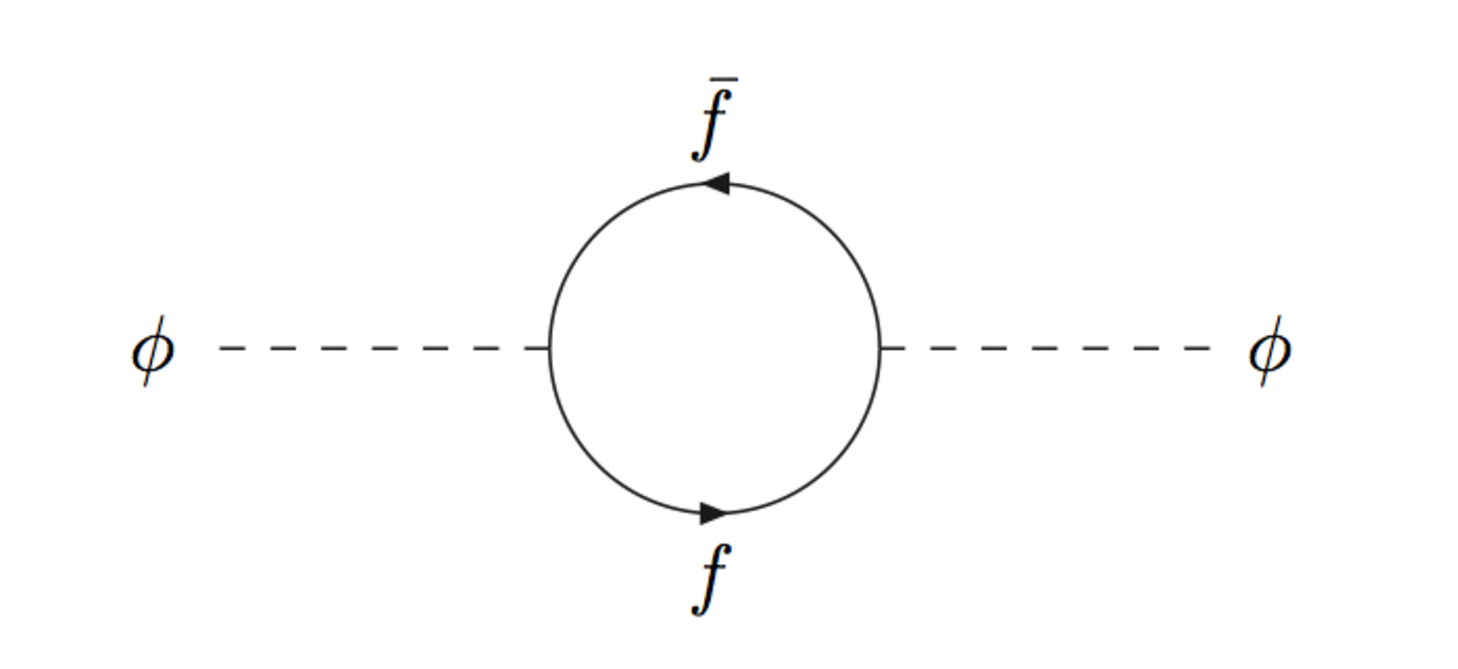
\includegraphics[scale=0.4]{figures/one-loop_diagram.pdf}
%\caption{}
%\label{fig: one-loop diagram}
%\end{subfigure}
%~%add desired spacing between images, e. g. ~, \quad, \qquad, \hfill etc.
%\begin{subfigure}[b]{0.45\textwidth}
%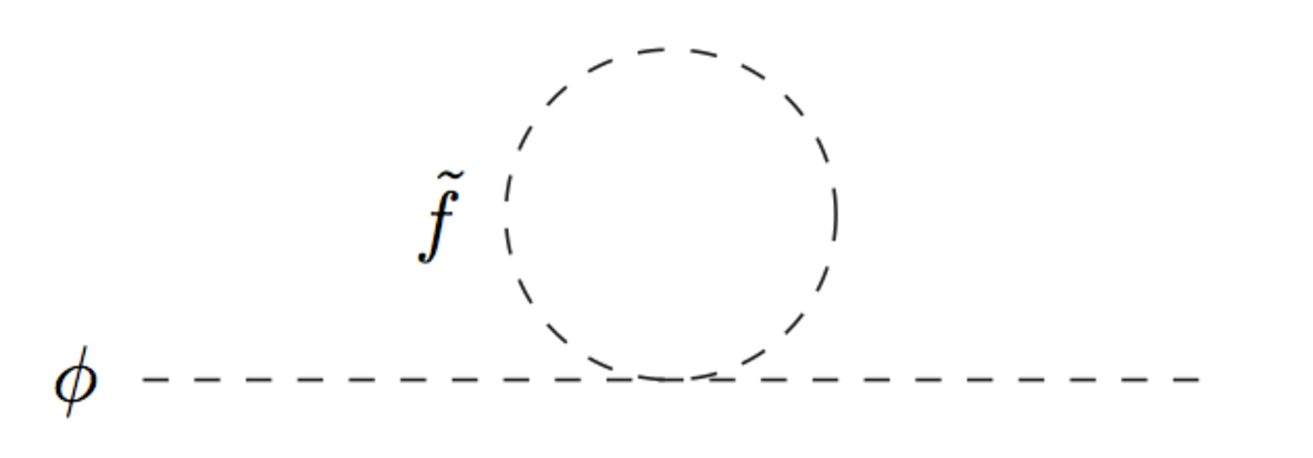
\includegraphics[scale=0.4]{figures/sfermion_one-loop_diagram.pdf}
%\caption{}
%\label{fig: sfermion_one-loop_diagram} 
%\end{subfigure}
%\caption{(a) A fermion and anti-fermion contribution to the self-energy of the Higgs boson in the Standard Model. (b) The sfermion loop contribution to the Higgs self-energy. $\widetilde{f}$ stands for sfermion.}
%\label{}
%\end{center}
%\end{figure}

The running coupling constants are functions of energy as shown in figure \ref{fig: running_coupling_constant}.
When energy increases, the strong coupling $\alpha_{3}$ and the weak coupling $\alpha_{2}$ go down, while the electromagnetic coupling $\alpha_{1}$ goes up.
In Grand Unified Theory (GUT), these three constants should be identical in strength when the energy is above the grand unification scale ($\approx 10^{16}$ GeV).
Although there is no direct evidence showing the coupling constants converge, the theorists still believe it is true.
However, these three constants do not converge in the Minimal Standard Model (MSM). 
If we extend the MSM into its supersymmetric version, Minimal Supersymmetric Standard Model (MSSM), they do converge well.
\begin{figure}[htbp]
\begin{center}
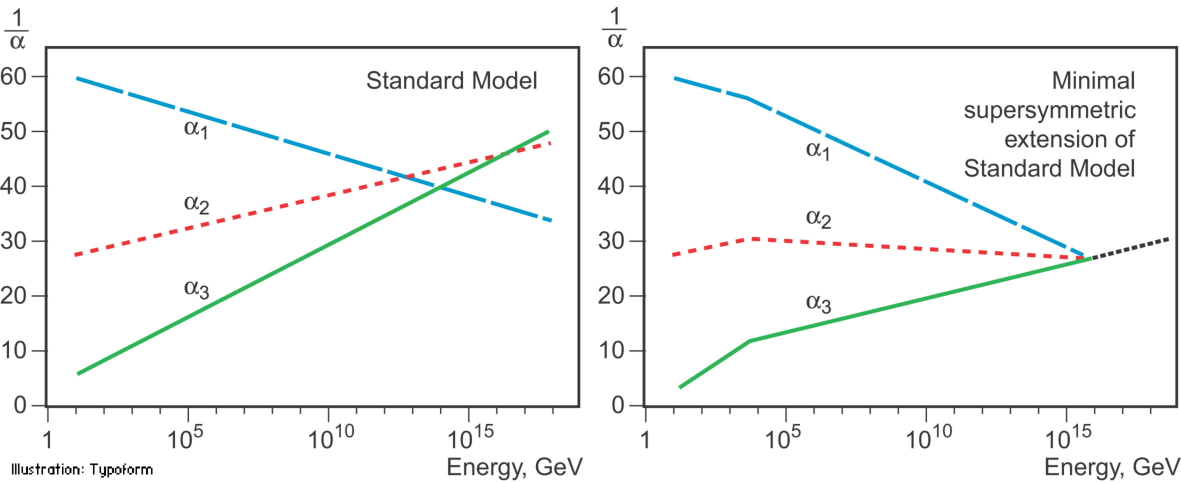
\includegraphics[scale=0.75]{figures/phypub4highen.pdf}
%This figure is from http://www.nobelprize.org/nobel_prizes/physics/laureates/2004/phypub4highen.jpg
\caption{The coupling constants at the GUT scale in the Minimal Standard Model (left) and in Minimal supersymmetric Standard Model (right) \cite{running_coupling_constants}.}
%Figure adapted from \url{http://www.nobelprize.org/nobel_prizes/physics/laureates/2004/phypub4highen.jpg}.}
\label{fig: running_coupling_constant}
\end{center}
\end{figure}

%Dark matter is expected to exist due to astronomical and cosmological effects and may consist of $80\%$ of the matter in our universe.
%Although dark matter cannot be seen directly with telescopes, it may be new particles which are not included in the SM.
%Many theorists predict the lightest SUSY particle (LSP) is stable and electrically neutral and interacts with the SM particles weakly.
%Because these are also the properties required for dark matter, SUSY provides potential candidates for dark matter.





%%%%%
%%%%%
%%%%%
\chapter{The Wess-Zumino model}
%\section{The Wess-Zumino model}


\section{Supersymmetry transformation}
%\subsection{Supersymmetry transformation}
If the equation of motion is invariant under a transformation, we call this is a symmetry transformation.
In other words, the action $S = \int d^{4}x \mathcal{L}$ is invariant under symmetry transformation.
There are two ways to keep the action S invariant: the Lagrangian $\mathcal{L}$ is either invariant or changes by a total derivative $\mathcal{L} \to \mathcal{L}' = \mathcal{L} + \partial_{\mu} \Lambda^{\mu}$ where we assume the quantity $\Lambda^{\mu}$ vanishes at the boundary.

%Let us consider a Lagrangian
%\begin{equation}
%\mathcal{L} = \frac{1}{2} (\partial_{\mu} A)^{2} + \frac{1}{2} (\partial_{\mu} B)^{2} + \frac{i}{2} \overline{\psi} \ \slashed{\partial} \psi + \frac{1}{2} (F^{2} + G^{2})
%\end{equation}
%where $A, B, F$, and $G$ are real scalar fields and $\psi$ is a 4-component Majorana spinor field.
%Wess and Zumino \cite{wess_and_zumino} defined an infinitesimal \textit{supersymmetry transformation} by
%%Wess and Zumino \cite{wess_and_zumino} defined an infinitesimal \textit{supersymmetry transformation}\footnote{It was called \textit{supergauge transformation} in the original paper written by Wess and Zumino.} by
%\begin{align}
%\delta A &= i \overline{\alpha} \gamma_{5} \psi ,\label{eq: 3.2}\\
%\delta B &= - \overline{\alpha} \psi ,\\
%\delta \psi &= -F \alpha + i G \gamma_{5} \alpha + \slashed{\partial} \gamma_{5} A \alpha + i \slashed{\partial} B \alpha ,\\
%\delta F &= i \overline{\alpha} \slashed{\partial} \psi ,\\
%\delta G &= \overline{\alpha} \gamma_{5} \slashed{\partial} \psi \label{eq: 3.6},
%\end{align}
%where the parameter $\alpha$ is an infinitesimal spinor which anticommutes with itself and with $\psi$ and commutes with the other fields.
%Although the Lagrangian is not itself invariant, it changes by a total derivative under a supersymmetry transformation providing an invariant action.
%
%We usually use complex fields $\mathcal{S}, \psi_{L}$ and $\mathcal{F}$ to replace the scalar fields and Majorana spinor field in Lagrangian
%\begin{equation}
%\mathcal{S} = \frac{1}{\sqrt{2}} (A + i B), \quad \psi_{L} = \frac{1 - \gamma_{5}}{2} \psi, \quad \mathcal{F} = \frac{1}{\sqrt{2}} (F + i G)
%\end{equation}
%then the SUSY transformations become
%\begin{align}
%\delta \mathcal{S} &= -i \sqrt{2} \overline{\alpha} \psi_{L} \label{eq: SUSY transformation 1}\\
%\delta \psi_{L} &= - \sqrt{2} \mathcal{F} \alpha_{L} + \sqrt{2} \slashed{\partial} \mathcal{S} \alpha_{R} \label{eq: SUSY transformation 2}\\
%\delta \mathcal{F} &= i \sqrt{2} \overline{\alpha} \slashed{\partial} \psi_{L} \label{eq: SUSY transformation 3} .
%\end{align}
%Thus, $\mathcal{S}, \psi_{L}$ and $\mathcal{F}$ transform into one another under the SUSY transformations.

The simplest example of a supersymmetric theory in four dimensions consists of a massless complex scalar boson field $\phi$ and its superpartner which is a massless left-handed two-component Weyl fermion $\psi$ without interactions between fields.
We can write down the simplest action immediately
\begin{align}
S &= \int d^{4} x \ (\mathcal{L}_{\mathrm{scalar}} + \mathcal{L}_{\mathrm{fermion}})\\
\mathcal{L}_{\mathrm{scalar}} &= \partial^{\mu} \phi^{*} \partial_{\mu} \phi, \quad \mathcal{L}_{\mathrm{fermion}} = i \psi^{\dag} \overline{\sigma}^{\mu} \partial_{\mu} \psi .
\end{align}
A SUSY transformation changes a boson field $\phi$ into a fermion field $\psi$.
The simplest infinitesimal transformation of the scalar fields is
\begin{equation} \label{eq: susy transformation for boson fields}
\delta \phi  = \epsilon \psi, \quad \delta \phi^{*} = \epsilon^{\dag} \psi^{\dag} ,
\end{equation}
where $\epsilon^{\alpha}$ is a constant, infinitesimal, anticommuting, two-component object with mass dimension $-\frac{1}{2}$.
Similarly, a fermion field is turned into a scalar field under SUSY transformation
\begin{equation} \label{eq: susy transformation for fermion fields}
\delta \psi_{\alpha} = -i (\sigma^{\mu} \epsilon^{\dag})_{\alpha} \partial_{\mu} \phi, \quad \delta \psi^{\dag}_{\dot{\alpha}} = i (\epsilon \sigma^{\mu})_{\dot{\alpha}} \partial_{\mu} \phi^{*} .
\end{equation}
%We can obtain the same transformation using equations (\ref{eq: 3.2}) to (\ref{eq: 3.6}) by setting $B = F = G =0$ and replacing $A \to \sqrt{2} \phi$ and $\psi \to \sqrt{2} \psi$ with a suitable choice of $\epsilon$.
The variations of the scalar and fermion Lagrangian are
\begin{align}
\delta \mathcal{L}_{\mathrm{scalar}} &= \partial^{\mu} (\delta \phi^{*}) \partial_{\mu} \phi + \partial^{\mu} \phi^{*} \partial_{\mu} (\delta \phi) \notag \\
&= \epsilon \partial^{\mu} \psi \partial_{\mu} \phi^{*} + \epsilon^{\dag} \partial^{\mu} \psi^{\dag} \partial_{\mu} \phi\\
%
\delta \mathcal{L}_{\mathrm{fermion}} &= i (\delta \psi^{\dag}) \overline{\sigma}^{\mu} \partial_{\mu} \psi + i \psi^{\dag} \overline{\sigma}^{\mu} \partial_{\mu} (\delta \psi) \notag \\
&= -\epsilon \sigma^{\nu} \partial_{\nu} \phi^{*} \overline{\sigma}^{\mu} \partial_{\mu} \psi + \psi^{\dag} \overline{\sigma}^{\mu} \sigma^{\nu} \epsilon^{\dag} \partial_{\mu} \partial_{\nu} \phi \notag \\
&= -\epsilon \partial^{\mu} \psi \partial_{\mu} \phi^{*} - \epsilon^{\dag} \partial^{\mu} \psi^{\dag} \partial_{\mu} \phi
+\partial_{\mu} (\epsilon \sigma^{\mu} \overline{\sigma}^{\nu} \psi \partial_{\nu} \phi^{*} - \epsilon \psi \partial^{\mu} \phi^{*} + \epsilon^{\dag} \psi^{\dag} \partial^{\mu}\phi) .
\end{align}
The sum of $\delta \mathcal{L}_{\mathrm{scalar}}$ and $\delta \mathcal{L}_{\mathrm{fermion}}$ gives a total derivative so the action is invariant.
Besides showing the action is invariant under SUSY transformation, we also need to show the SUSY algebra closes.
However, equations (\ref{eq: susy transformation for boson fields}) and (\ref{eq: susy transformation for fermion fields}) only valid for on-shell, which means $\overline{\sigma}^{\mu} \partial_{\mu} \psi = 0$.
We have to introduce a new complex scalar field $F$, called the auxiliary field. %, with a mass dimension of 2.
The Lagrangian of the auxiliary field is defined as $\mathcal{L}_{\mathrm{auxiliary}} = F^{*} F$.
The auxiliary field transforms under SUSY as
\begin{equation}
\delta F = - i \epsilon^{\dag} \overline{\sigma}^{\mu} \partial_{\mu} \psi, \quad 
\delta F^{*} = i \partial_{\mu} \psi^{\dag} \overline{\sigma}^{\mu} \epsilon
\end{equation}
and equation (\ref{eq: susy transformation for fermion fields}) has to be modified to
\begin{equation}
\delta \psi_{\alpha} = -i (\sigma^{\mu} \epsilon^{\dag})_{\alpha} \partial_{\mu} \phi + \epsilon_{\alpha} F, \quad 
\delta \psi^{\dag}_{\dot{\alpha}} = i (\epsilon \sigma^{\mu})_{\dot{\alpha}} \partial_{\mu} \phi^{*} + \epsilon^{\dag}_{\dot{\alpha}} F^{*}.
\end{equation}
Then we can show that fields $X = \phi, \phi^{*}, \psi, \psi^{\dag}, F, F^{*}$ satisfies
\begin{equation}
(\delta_{\epsilon2} \delta_{\epsilon1} - \delta_{\epsilon1} \delta_{\epsilon2}) X = i (- \epsilon_{1} \sigma^{\mu} \epsilon^{\dag}_{2} + \epsilon_{2} \sigma^{\mu} \epsilon^{\dag}_{1}) \partial_{\mu} X
\end{equation}
and keeps the Lagrangian $\mathcal{L}_{\mathrm{scalar}} + \mathcal{L}_{\mathrm{fermion}} + \mathcal{L}_{\mathrm{auxiliary}}$ invariant under SUSY transformation for the off-shell case.

%Since SUSY is a kind of symmetry, we can find the conserved supercurrents and construct the conserved supercharges from Noether's theorem
%\begin{align}
%& J^{\mu}_{\alpha} = (\sigma^{\nu} \overline{\sigma}^{\mu} \psi)_{\alpha} \partial_{\nu} \phi^{*}, \quad 
%J^{\dag \mu}_{\dot{\alpha}} = ( \psi^{\dag} \overline{\sigma}^{\mu} \sigma^{\nu})_{\dot{\alpha}} \partial_{\nu} \phi\\
%%
%& Q_{\alpha} = \sqrt{2} \int d^{3}x \ J^{0}_{\alpha}, \quad 
%Q^{\dag}_{\dot{\alpha}} = \sqrt{2} \int d^{3}x J^{\dag 0}_{\dot{\alpha}} .
%\end{align}
%The supercharges play the role of generators of SUSY transformations and obey the commutation relations mentioned in section \ref{sec: supermultiplets}.



\section{Supersymmetric Lagrangian with interactions}
%\subsection{Supersymmetric Lagrangian with interactions}
We have considered the free Lagrangian defined as
\begin{equation} \label{eq: free Lagrangian}
\mathcal{L}_{\mathrm{free}} = \partial^{\mu} \phi^{*i} \partial_{\mu} \phi_{i} + i \psi^{\dag i} \overline{\sigma}^{\mu} \partial_{\mu} \psi_{i} + F^{*i} F_{i} \quad,
\end{equation}
now let us consider the realistic theory which contains the interactions between fields.
The general non-gauge interaction Lagrangian for chiral supermultiplets can be written as \footnote{c.c stands for complex conjugate.}
\begin{equation} \label{eq: non-gauge interaction Lagrangian}
\mathcal{L}_{\mathrm{int}} = \Big( - \frac{1}{2} W^{ij} \psi_{i} \psi_{j} + W^{i} F_{i}\Big) + \mathrm{c.c}
\end{equation}
where $W^{i}$ and $W^{ij}$ are defined as
\begin{equation}
W^{i} \equiv \frac{\partial W}{\partial \phi_{i}}% = M^{ij} \phi_{j} + \frac{1}{2} y^{ijk} \phi_{j} \phi_{k}.
\quad
W^{ij} \equiv \frac{\partial W}{\partial \phi_{i} \partial \phi_{j}}
\end{equation}
and W is the superpotential which is defined as
\begin{equation}
W = \frac{1}{2} M^{ij} \phi_{i} \phi_{j} + \frac{1}{6} y^{ijk} \phi_{i} \phi_{j} \phi_{k} .
\end{equation}


The auxiliary fields $F_{i}$ and $F^{*i}$ can be replaced using equations of motion.
From equations (\ref{eq: free Lagrangian}) and (\ref{eq: non-gauge interaction Lagrangian}), we find the part of the $\mathcal{L}_{\mathrm{free}} + \mathcal{L}_{\mathrm{int}}$ contains the auxiliary fields is $F^{*i} F_{i} + W^{i} F_{i} + W^{*}_{i} F^{*i}$, leading to the equations of motion
\begin{equation} \label{eq: auxiliary field F}
F_{i} = - W^{*}_{i}, \quad 
F^{*i} = - W^{i} .
\end{equation}
Thus the Lagrangian becomes
\begin{align} \label{eq: Lagrangian with interaction}
%\mathcal{L} &= \mathcal{L}_{\mathrm{free}} + \mathcal{L}_{\mathrm{int}} \notag \\
\mathcal{L}_{\mathrm{free}} + \mathcal{L}_{\mathrm{int}} 
&= \partial^{\mu} \phi^{*i} \partial_{\mu} \phi_{i} + i \psi^{\dag i} \overline{\sigma}^{\mu} \partial_{\mu} \psi_{i} -\frac{1}{2} \Big( W^{ij} \psi_{i} \psi_{j} + W^{*}_{ij} \psi^{\dag i} \psi^{\dag j} \Big) - W^{i} W^{*}_{i} .
\end{align}
From equations (\ref{eq: auxiliary field F}) and (\ref{eq: Lagrangian with interaction}), we know the scalar potential is given in terms of superpotential by
\begin{equation}
V(\phi, \phi^{*}) = W^{i}W^{*}_{i} = F^{*i} F_{i}
\end{equation}
which is non-negative.


%%%%%
%%%%%
%%%%%
\chapter{Superspace and superfields}
%\section{Superspace and superfields}
The supersymmetric formalism can be recast in an elegant way by introducing superspace and superfields.
A superspace is described by the four ordinary space-time coordinates $x^{\mu}$ and four anticommuting Grassmannian coordinates $\theta_{\alpha}$ and $\overline{\theta}_{\dot{\alpha}}$, where the spinor indices $\alpha = 1, 2$ and $\dot{\alpha} = 1, 2$.
A superfield is a function of superspace coordinates: $S (x^{\mu}, \theta_{\alpha}, \overline{\theta}_{\dot{\alpha}})$, which contains bosonic, fermonic and auxiliary fields in the corresponding supermultiplet.



\section{Superspace}
%\subsection{Superspace}
Since $\theta_{\alpha}$ and $\overline{\theta}_{\dot{\alpha}}$ anticommute among themselves, any product cannot contain more than two $\theta$'s or more than two $\overline{\theta}$'s.
A general superfield can be expanded in terms of $\theta$ and $\overline{\theta}$
\begin{equation}
S(x, \theta, \overline{\theta}) = a + \theta \xi + \overline{\theta} \overline{\chi} + \theta \theta b + \overline{\theta} \overline{\theta} c + \overline{\theta} \overline{\sigma}^{\mu} \theta v_{\mu} + \theta \theta \overline{\theta} \overline{\zeta} + \overline{\theta} \overline{\theta} \theta \eta + \theta \theta \overline{\theta} \overline{\theta} d
\end{equation}
where all spinor indices are suppressed.
The 8 bosonic component fields $a, b, c, d$, and $v_{\mu}$ and 4 two-component fermion component fields $\xi, \overline{\chi}, \eta, \overline{\zeta}$ are complex functions of $x^{\mu}$.
To formulate SUSY transformation in superspace, we define the SUSY generators 
\footnote{We also can define 
$Q^{\alpha} = i \frac{\partial}{\partial \theta_{\alpha}} + (\overline{\theta} \overline{\sigma}^{\mu})^{\alpha} \partial_{\mu}$ and 
$\overline{Q}^{\dot{\alpha}} = -i \frac{\partial}{\partial \overline{\theta}_{\dot{\alpha}}} - (\overline{\sigma}^{\mu} \theta)^{\dot{\alpha}} \partial_{\mu}$}
\begin{equation}
Q_{\alpha} = -i \frac{\partial}{\partial \theta^{\alpha}} - \sigma^{\mu}_{\alpha \dot{\beta}} \overline{\theta}^{\dot{\beta}} \partial_{\mu}, \quad 
\overline{Q}_{\dot{\alpha}} = i \frac{\partial}{\partial \overline{\theta}^{\dot{\alpha}}} + \theta^{\beta} \sigma^{\mu}_{\beta \dot{\alpha}} \partial_{\mu}
\end{equation}
and they follow the commutation relations
\begin{align}
& \{Q_{\alpha}, \overline{Q}_{\dot{\beta}}\} = 2 \sigma^{\mu}_{\alpha \dot{\beta}} P_{\mu} = -2i \sigma^{\mu}_{\alpha \dot{\beta}} \partial_{\mu} \\
& \{Q_{\alpha}, Q_{\beta}\} = 0, \quad 
\{\overline{Q}_{\dot{\alpha}}, \overline{Q}_{\dot{\beta}}\} = 0 .
\end{align}
Then the infinitesimal SUSY transformation can be written as
\begin{align}
\delta_{\epsilon} S(x, \theta, \overline{\theta}) &= S(x^{\mu} + i \epsilon \sigma^{\mu}\overline{\theta} + i \overline{\epsilon} \overline{\sigma}^{\mu} \theta, \theta + \epsilon, \overline{\theta} + \overline{\epsilon}) - S(x, \theta, \overline{\theta})\\
&= (i \epsilon Q + i \overline{\epsilon} \overline{Q}) S(x, \theta, \overline{\theta})\\
&= \Big[ \epsilon^{\alpha} \frac{\partial}{\partial \theta^{\alpha}} + \overline{\epsilon}_{\dot{\alpha}} \frac{\partial}{\partial \overline{\theta}_{\dot{\alpha}}} - i \big( \epsilon \sigma^{\mu} \overline{\theta} + \overline{\epsilon} \overline{\sigma}^{\mu} \theta \big)  \Big] S(x, \theta, \overline{\theta})
\end{align}
Now we introduce SUSY covariant derivatives $D_{\alpha}$ and $\overline{D}_{\dot{\alpha}}$ that anticommute with SUSY generators $Q$ and $\overline{Q}$
\begin{equation}
D_{\alpha} = \frac{\partial}{\partial \theta^{\alpha}} + i \sigma^{\mu}_{\alpha \dot{\beta}} \overline{\theta}^{\dot{\beta}} \partial_{\mu}, \quad 
\overline{D}_{\dot{\alpha}} = (D_{\alpha})^{\dag} = \frac{\partial}{\partial \overline{\theta}^{\dot{\alpha}}} + i \theta^{\beta} \sigma^{\mu}_{\beta \dot{\alpha}} \partial_{\mu}
\end{equation}
with the commutation relations
\begin{align*}
& \{ D_{\alpha}, \overline{D}_{\dot{\beta}}\} = 2i \sigma^{\mu}_{\alpha \dot{\beta}} \partial_{\mu}, \quad \{ D_{\alpha}, D_{\beta}\} = \{ \overline{D}_{\dot{\alpha}}, \overline{D}_{\dot{\beta}}\} = 0\\
& \{ D_{\alpha}, Q_{\beta} \} = \{ D_{\alpha}, \overline{Q}_{\dot{\beta}}\} = \{ \overline{D}_{\dot{\alpha}}, Q_{\beta} \} = \{ \overline{D}_{\dot{\alpha}}, \overline{Q}_{\dot{\beta}}\} = 0  
\end{align*}
Then we can find $\delta_{\epsilon} (D_{\alpha} S) = D_{\alpha} (\delta_{\epsilon} S)$ and $\delta_{\epsilon} (\overline{D}_{\dot{\alpha}} S) = \overline{D}_{\dot{\alpha}} (\delta_{\epsilon} S)$.



\section{Chiral superfields}
%\subsection{Chiral superfields}
The chiral superfields, which are irreducible representations of the SUSY algebra, can describe spin 0 bosons and spin 1/2 fermions -- for example, the Higgs boson and the quarks and leptons.
A superfield $\Phi (x, \theta, \overline{\theta})$ satisfies the condition
\begin{equation} \label{eq: definition of chiral superfield}
\overline{D}_{\dot{\alpha}} \Phi =0
\end{equation}
 is called a chiral (or left-chiral) superfield.\footnote{The complex conjugate of $\Phi$, which is denoted as $\Phi^{*}$, is called antichiral (or right-chiral) superfield and satisfies
\begin{equation} \label{eq: definition of antichiral superfield}
D_{\alpha} \Phi^{*} = 0.
\end{equation}
}
 %and its complex conjugate $\Phi^{*}$ is called antichiral (or right-chiral) superfield and satisfies
%\begin{equation} \label{eq: definition of antichiral superfield}
%D_{\alpha} \Phi^{*} = 0.
%\end{equation}
If we define the chiral coordinates $(y^{\mu}, \theta)$ and antichiral coordinates $(\overline{y}^{\mu}, \overline{\theta})$, where
\begin{equation}
y^{\mu} = x^{\mu} + i \theta \sigma^{\mu} \overline{\theta}, \quad 
\overline{y}^{\mu} = x^{\mu} - i \theta \sigma^{\mu} \overline{\theta}
\end{equation}
and the covariant derivative in (anti)chiral coordinates becomes
\begin{equation}
D_{\alpha} = \frac{\partial}{\partial \theta^{\alpha}} + 2 i \sigma^{\mu}_{\alpha \dot{\beta}} \overline{\theta}^{\dot{\beta}} \frac{\partial}{\partial y^{\mu}}, \quad 
\overline{D}_{\dot{\alpha}} = \frac{\partial}{\partial \overline{\theta}^{\dot{\alpha}}} .
\end{equation}
then the general form of a chiral superfield is a function of $y^{\mu}$ and $\theta$ only.
We can get ride of the $\overline{\theta}$ dependence in the chiral coordinates $(y^{\mu}, \theta)$.
Hence the general form of a chiral superfield can be expanded as
\begin{equation}
\Phi (y, \theta) = \phi (y) + \sqrt{2} \theta \psi (y) + \theta \theta F(y) .
\end{equation}
By applying SUSY transformation on the chiral superfield $\Phi$, through this $\delta_{\epsilon} \Phi = (i \epsilon Q + i \overline{\epsilon} \overline{Q}) \Phi$, the component fields are found to be
\begin{align} 
\delta_{\epsilon} \phi &= \sqrt{2} \epsilon \psi \label{eq: SUSY transformation 4}\\
\delta_{\epsilon} \psi_{\alpha} &= i \sqrt{2}  \partial_{\mu} \phi (\sigma^{\mu} \overline{\epsilon})_{\alpha} - \sqrt{2} \epsilon_{\alpha} F \label{eq: SUSY transformation 5}\\
\delta_{\epsilon} F &= i \sqrt{2}  \partial_{\mu} \psi \sigma^{\mu} \overline{\epsilon} \label{eq: SUSY transformation 6}.
\end{align}
%in agreement with equations (\ref{eq: SUSY transformation 1}), (\ref{eq: SUSY transformation 2}), and (\ref{eq: SUSY transformation 3}), up to a multiplicative.



\section{Vector superfields}
%\subsection{Vector superfields}
In order to describe the spin 1 gauge bosons, we have to introduce the vector (real) superfields $V$ which are defined as
\begin{equation}
V(x, \theta, \overline{\theta}) = V^{\dag} (x, \theta, \overline{\theta}) .
\end{equation}
The general vector superfield $V(x, \theta, \overline{\theta})$ has the expansion
\begin{align}
V(x, \theta, \overline{\theta}) &= C + i \theta \chi - i \overline{\theta} \overline{\chi} + \theta \sigma^{\mu} \overline{\theta} v_{\mu} + \frac{i}{2} \theta \theta (M + iN) - \frac{i}{2} \overline{\theta} \overline{\theta} (M - iN) \notag \\
& + i \theta \theta \overline{\theta} (\overline{\lambda} + \frac{i}{2} \overline{\sigma}^{\mu} \partial_{\mu} \chi ) - i \overline{\theta} \overline{\theta} \theta (\lambda - \frac{i}{2} \sigma^{\mu} \partial_{\mu} \overline{\chi}) + \frac{1}{2} \theta \theta \overline{\theta} \overline{\theta} (D - \frac{1}{2} \partial^{2} C)
\end{align}
where $C, M, N$, and $D$ are real scalars, $\chi$ and $\lambda$ are Weyl spinors, and $v^{\mu}$ is a vector field.
Since there are too many component fields in a single supermultiplet, we want to reduce the number of them.
Consider an abelian SUSY gauge transformation for a vector superfield
\begin{equation}
%V \to V + i (\Lambda - \Lambda^{\dag})
V \to V + i (\Phi - \Phi^{\dag})
\end{equation}
where the gauge transformation parameter $\Phi$ is a chiral superfield. Then the component fields $C, \chi, M, N$ and one component of $v_{\mu}$ can be gauged away.
This is called Wess-Zumino gauge.
By introducing Wess-Zumino gauge, we can reduce the number of components of the vector superfield as
\begin{equation} \label{eq: WZ gauge vector superfield}
V_{WZ} = \theta \sigma^{\mu} \overline{\theta} v_{\mu}(x) + i \theta \theta \overline{\theta} \overline{\lambda}(x) - i \overline{\theta} \overline{\theta} \theta \lambda(x) + \frac{1}{2} \theta \theta \overline{\theta} \overline{\theta} D(x) .
\end{equation}
Since there is at least one $\theta$ in the $V_{WZ}$, the only non-vanishing power of $V_{WZ}$ is
\begin{equation}
V^{2}_{WZ} = \big[ \theta \sigma^{\mu} \overline{\theta} v_{\mu}(x) \big] \big[ \theta \sigma^{\nu} \overline{\theta} v_{\nu}(x) \big] = \frac{1}{2} \theta \theta \overline{\theta} \overline{\theta} v_{\mu} v^{\mu}
\end{equation}
and $V^{n}_{WZ} = 0, n \ge 3$.









%%%%%
%%%%%
%%%%%
\chapter{Supersymmetry breaking}
%\section{Supersymmetry breaking}

%As mentioned in section \ref{sec: supermultiplets}, all particles belonging to the same supermultiplet have the same mass.
SUSY theory says that all particles belonging to the same supermultiplet have the same mass.
That is to say, the masses of SM particles and their superpartners are identical.
However, it is not true in reality because we didn't find any sparticles, for example, there is no selectron with mass 0.51 MeV and a massless fermionic partner of the photon.
Hence the supersymmetry must be spontaneously broken.



\section{Vacuum expectation value in SUSY}
%\subsection{Vacuum expectation value in SUSY}
The superalgebra tells us the anticommutation relation $\{ Q_{\alpha}, \overline{Q}_{\dot{\beta}} \} = 2 \sigma^{\mu}_{\alpha \dot{\beta}} P_{\mu}$.
So we have
\begin{align}
\{ Q_{1}, \overline{Q}_{1} \} = 2 ( P_{0} + P_{3}) \notag \\
\{ Q_{2}, \overline{Q}_{2} \} = 2 ( P_{0} - P_{3}) 
\end{align}
Then the Hamiltonian for SUSY is given by
\begin{equation}
H \equiv P^{0} = \frac{1}{4} (\{ Q_{1}, \overline{Q}_{1} \}  + \{ Q_{2}, \overline{Q}_{2} \} ) .
\end{equation}
It follows that the expectation value of the Hamiltonian for an arbitrary state $| \Psi \rangle$ is a sum of squares and therefore non-negative
\begin{equation}
E_{\Psi} = \langle \Psi | H | \Psi \rangle = \frac{1}{4} \sum_{\alpha} ( \| Q_{\alpha} | \Psi \rangle \|^2 + \| \overline{Q}_{\dot{\alpha}} | \Psi \rangle \|^2 ) \ge 0 .
\end{equation}
For a vacuum state (ground state) $|\Psi \rangle = | \Omega \rangle$, $E = 0$ if and only if $Q_{\alpha} | \Omega \rangle = \overline{Q}_{\dot{\alpha}} | \Omega \rangle = 0$.
If a ground state has non-vanishing positive energy, the SUSY is broken spontaneously. 



\section{The $F$-term breaking and $D$-term breaking}
%\subsection{The $F$-term breaking and $D$-term breaking}
A state $| \Omega \rangle$ is called a vacuum state when the scalar potential $V$ has a minimum.
There are two kinds of vacuums, the true vacuum and the false vacuum.
If the minimum of $V$ is the global minimum, then the vacuum is the true vacuum; otherwise it is a false vacuum.
%The scalar potential is given in (\ref{eq: scalar potential})
The scalar potential is
\begin{equation}
V(\phi, \phi^{*}) = F^{*i} F_{i} + \frac{1}{2} \sum_{a} D^{a} D_{a} \ge 0 \notag
\end{equation}
where $D_{a}$ is a real bosonic auxiliary field. \footnote{For more details about $D^{a}$, refers to appendix \ref{app: supersymmetric gauge theories}.}
%and it is non-negative. 
It is clear that when $F_{i} = D_{a} = 0$ then $V = 0$ is a global minimum.

Consider the SUSY transformation in equations (\ref{eq: SUSY transformation 4}), (\ref{eq: SUSY transformation 5}), (\ref{eq: SUSY transformation 6}), SUSY is broken if one of the $\delta \phi$, $\delta \psi$, $\delta F \neq 0$.
Since a vacuum state is Lorentz invariant which implies all the space-time derivatives and all non-scalar fields must vanish.
SUSY breaking conditions can be recast as $\langle F \rangle \neq 0$ which is called $F$-term breaking.
%Similarly, for a vector superfield $V(\lambda, A_{\mu}, D)$, the SUSY breaking condition is $\langle D \rangle \neq 0$ because $\delta \lambda \propto \epsilon D$.
%And this is called $D$-term breaking.

Now let's consider the simplest model, the O'Raifeartaigh model \cite{O_Raifeartaigh},  of SUSY breaking. Given three chiral supermultiplets $\phi_{1}$, $\phi_{2}$, and $\phi_{3}$, the K\"{a}hler potential and superpotential are 
\begin{equation}
K = \phi^{\dag}_{i} \phi_{i}, \quad
W = g \phi_{1} ( \phi^{2}_{3} - m^{2}) + M \phi_{2} \phi_{3}, \quad
M \gg m
\end{equation}
From (\ref{eq: auxiliary field F}), we can find the auxiliary fields are
\begin{align}
F^{*1} &= - W^{1} = \frac{\partial W}{\partial \phi_{1}} = g ( \phi^{2}_{3} - m^{2})\\
F^{*2} &= - W^{2} = \frac{\partial W}{\partial \phi_{2}} = M \phi_{3}\\
F^{*3} &= - W^{3} = \frac{\partial W}{\partial \phi_{3}} = 2 g \phi_{1} \phi_{3} + M \phi_{2} .
\end{align}
It is impossible to have $F^{*i} = 0$ simultaneously because $F^{*2} = 0$ contradicts to $F^{*1} = 0$.
Therefore SUSY must break.





%%%%%
%%%%%
%%%%%
\chapter{The minimal supersymmetry standard model}
%\section{The minimal supersymmetry standard model}
The Minimal Supersymmetry Standard Model (MSSM) is a supersymmetrization of the SM by introducing SUSY partners to every particle in the SM spectrum. 
The key word ``minimal" means that we want to keep the number of superfields and interactions as small as possible. 



\section{The particle content of the MSSM}
%\subsection{The particle content of the MSSM}
In the MSSM, the vector fields of the SM are assigned to vector supermultiplets and the matter fields of the SM are assigned to chiral supermultiplets.
The scalar superpartners of fermions are called \textit{squarks} and \textit{sleptons} or collectively called \textit{sfermions}, where the prefix `\textit{s}' stands for scalar.
For the fermionic superpartners of bosons, we append ``-ino" to the SM particles.
We usually add a tilde ($\widetilde{ \quad }$) on the symbol of a SM particle to denote its superpartner.

The SM fermions are described by five left-chiral superfields: $Q_{i}$ contains the (s)quark $SU(2)$ doublets, $\overline{u}_{i}$  and $\overline{d}_{i}$ contain the (s)quark singlets \footnote{The $SU(2)$ singlet super fields contain left-handed antifermions.}, $L_{i}$ contains the (s)lepton doublets, and $\overline{e}_{i}$ contains the (s)lepton singlets.
The index $i = 1, 2, 3$ is the generation index because there are 3 generations of SM particles.

We introduce vector supermultiplets to describe the gauge sector of the SM.
The fermonic superpartners of the gauge bosons are generally referred to as \textit{gauginos} which include 8 glunios $\widetilde{g}$ as superpartners of 8 gluons of QCD, three winos $\widetilde{W}^{+}$, $\widetilde{W}^{0}$, $\widetilde{W}^{-}$ as superpartners of the $SU(2)_{L}$ gauge bosons, and a bino $\widetilde{B}^{0}$ as $U(1)_{Y}$ gaugino.
%There are 8 glunios $\widetilde{g}$ as superpartners of 8 gluons of QCD, three winos $\widetilde{W}^{+}$, $\widetilde{W}^{0}$, $\widetilde{W}^{-}$ as superpartners of the $SU(2)_{L}$ gauge bosons, and a bino $\widetilde{B}^{0}$ as $U(1)_{Y}$ gaugino.
Since the $W^{0}$ and $B^{0}$ gauge eigenstates mix to give mass eigenstates $Z^{0}$ and $\gamma$ after the electroweak symmetry breaking, the corresponding gaugino mixtures are called zinos $\widetilde{Z}^{0}$ and photinos $\widetilde{\gamma}$.

Since the Higgs scalar boson has spin $0$, it must be described by a chiral supermultiplet.
For the fermionic partner of a Higgs chiral supermultiplet, we introduce two weak isospin doublets with weak hypercharge $Y = \frac{1}{2}$ and $Y = -\frac{1}{2}$.
There are two main reasons to have two Higgs supermultiplets.
If there were only one Higgs supermultiplet, the model will suffer from quadratic divergence because the condition for cancellation of gauge anomalies $Tr(T^{2}_{3} Y) = Tr(Y^{3}) = 0$ isn't satisfied.
However, the total contributions to the anomaly traces from two Higgs supermultiplets, one with each $Y = \pm \frac{1}{2}$, can cancel.
The other reason is that it is impossible to give masses to both up-type quarks \footnote{The up-type quarks are up, charm, and top quark.} and down-type quarks \footnote{The down-type quarks are down, strange, and bottom quark.} if there were only one Higgs supermultiplet.
The two complex scalar fields are called $H_{u}$ (with $Y = \frac{1}{2}$) and $H_{d}$ (with $Y = -\frac{1}{2}$).
Because the electric charge is the summation of the third component of weak isospin and the weak hypercharge, the components of $H_{u}$ and $H_{d}$ with $T_{3} = (\frac{1}{2}, -\frac{1}{2})$ are denoted as $(H^{+}_{u}, H^{0}_{u})$ and $(H^{0}_{d}, H^{-}_{d})$.

Table \ref{table: chiral supermultiplets in the MSSM} and table \ref{table: gauge supermultiplets in the MSSM} summarise the chiral and gauge supermultiplets in the MSSM.
In these two tables, the `bar' on the fields is merely a label, signifying `antiparticles'.%, and does not denote Dirac conjugation.
The unbarred fields are the left-handed pieces of a Dirac spinor and barred fields the conjugate of the right-handed pieces of a Dirac spinor.
For example, $e$ stands for $e_{L}$ and $\overline{e}$ stands for $e^{\dag}_{R}$.
They form a Dirac spinor
\begin{equation}
\left( \begin{array}{c} e_{L}\\ {e}_{R} \end{array} \right) = \left( \begin{array}{c} e\\ \overline{e}^{\dag} \end{array} \right)
\end{equation}


\begin{table}[htdp]
\begin{center}
{\renewcommand{\arraystretch}{1.5}%vertical spacing
\begin{tabular}{|c|c|c|c|c|}
\hline
\multicolumn{2}{|c|}{Names} & spin 0 & spin 1/2 & $SU(3)_{C}$, $SU(2)_{L}$, $U(1)_{Y}$\\
\hline
\hline
\multirow{3}{3cm}{squarks, quarks ($\times 3$ families)} &Q & ($\widetilde{u}_{L}$, \quad $\widetilde{d}_{L})$ & $(u_{L}, \quad d_{L})$ & $(\mathbf{3}, \quad \mathbf{2}, \quad \frac{1}{6})$\\
& $\overline{u}$ & $\widetilde{\overline{u}}_{L} = \widetilde{u}^{*}_{R}$ & $\overline{u}_{L} = u^{\dag}_{R}$ & $(\overline{\mathbf{3}}, \quad \mathbf{1}, \quad -\frac{2}{3})$\\
& $\overline{d}$ & $\widetilde{\overline{d}}_{L}= \widetilde{d}^{*}_{R}$ & $\overline{d}_{L} =d^{\dag}_{R}$ & $(\overline{\mathbf{3}}, \quad \mathbf{1}, \quad \frac{1}{3})$\\
\hline
\multirow{2}{3cm}{sleptons, leptons ($\times 3$ families)} & L & $(\widetilde{\nu}, \quad \widetilde{e}_{L})$ & $(\nu, \quad e_{L})$ & $(\mathbf{1}, \quad \mathbf{2}, \quad -\frac{1}{2})$\\
& $\overline{e}$ & $\widetilde{\overline{e}}_{L} =\widetilde{e}^{*}_{R}$ & $\overline{e}_{L} = e^{\dag}_{R}$ & $(\mathbf{1}, \quad \mathbf{1}, \quad 1)$\\
\hline
\multirow{2}{*}{Higgs, higgsinos} & $H_{u}$ & $(H^{+}_{u}, \quad H^{0}_{u})$ & $(\widetilde{H}^{+}_{u}, \quad \widetilde{H}^{0}_{u})$ & $(\mathbf{1}, \quad \mathbf{2}, \quad +\frac{1}{2})$\\
& $H_{d}$ & $(H^{0}_{d}, \quad H^{-}_{d})$ & $(\widetilde{H}^{0}_{d}, \quad \widetilde{H}^{-}_{d})$ & $(\mathbf{1}, \quad \mathbf{2}, \quad -\frac{1}{2})$\\
\hline
\end{tabular}
}% end of \renewcommand{}
\end{center}
\caption{Chiral supermultiplet fields in the MSSM}
\label{table: chiral supermultiplets in the MSSM}
\end{table}%

\begin{table}[htdp]
\begin{center}
{\renewcommand{\arraystretch}{1.5}%vertical spacing
\begin{tabular}{|c|c|c|c|}
\hline
Names & spin 1/2 & spin 1 & $SU(3)_{C}, SU(2)_{L}, U(1)_{Y}$\\ 
\hline
\hline
gluino, gluon & $\widetilde{g}$ & $g$ & $(\mathbf{8}, \quad, \mathbf{1}, \quad 0)$\\
\hline
winos, $W$ bosons & $\widetilde{W}^{\pm}$, $\widetilde{W}^{0}$ & $W^{\pm}$, $W^{0}$ & $(\mathbf{1}, \quad \mathbf{3}, \quad 0)$\\
\hline
bino, $B$ boson & $\widetilde{B}^{0}$ & $B^{0}$ & $(\mathbf{1}, \quad \mathbf{1}, \quad 0)$\\
\hline
\end{tabular}
} % end of \renewcommand{}
\end{center}
\caption{Gauge supermultiplet fields in the MSSM}
\label{table: gauge supermultiplets in the MSSM}
\end{table}%



\section{The superpotential of MSSM}
%\subsection{The superpotential of MSSM}
The superpotential of the MSSM is
\begin{equation} \label{eq: superpotential in MSSM}
W_{\mathrm{MSSM}} = \sum^{3}_{i, j = 1} (\mathbf{y_{u}})_{ij} H_{u} Q_{i} \overline{u}_{j} - (\mathbf{y_{d}})_{ij} H_{d} Q_{i} \overline{d}_{j} - (\mathbf{y_{e}})_{ij} H_{d} L_{i} \overline{e}_{j} +  \mu H_{u} H_{d}
\end{equation}
where $i$ and $j$ are generation indecies and the dimensionless Yukawa couplings $\mathbf{y_{u}}$, $\mathbf{y_{d}}$, $\mathbf{y_{e}}$ are $3 \times 3$ matrices in family (generation) space.
The colour indices have been suppressed, so that $Q_{i} \overline{u}_{j}$ is really $Q^{\alpha}_{i} \overline{u}_{\alpha j}$ where the superscript $\alpha = 1, 2, 3$ is the colour $\mathbf{3}$ (triplet) index and the subscript $\alpha$ is $\overline{\mathbf{3}}$ (anti-triplet) index.
In the superpotential , $W_{\mathrm{MSSM}}$, the first three terms give the mass to up quarks, down quarks and leptons via Yukawa couplings.
And the $\mu$-term, which is the supersymmetric version of the Higgs boson mass in the SM, is defined as $\mu H_{u} H_{d} = \mu (H_{u})_{\alpha} (H_{d})_{\beta} \epsilon^{\alpha \beta}$.

For example, since the top quark, bottom quark, and $\tau$ lepton are the heaviest fermions in the SM, we can consider an approximation that only the $(3, 3)$ components of $\mathbf{y_{u}}$, $\mathbf{y_{d}}$, and $\mathbf{y_{e}}$ are non-zero.
\begin{equation}
\mathbf{y_{u}} \approx \left( \begin{array}{ccc} 0 & 0 & 0\\ 0 & 0 & 0\\ 0 & 0 & y_{t} \end{array}\right), \quad
\mathbf{y_{d}} \approx \left( \begin{array}{ccc} 0 & 0 & 0\\ 0 & 0 & 0\\ 0 & 0 & y_{b} \end{array}\right), \quad
\mathbf{y_{e}} \approx \left( \begin{array}{ccc} 0 & 0 & 0\\ 0 & 0 & 0\\ 0 & 0 & y_{\tau} \end{array}\right)
\end{equation}
The superpotential $W$ is
\begin{align}
W_{\mathrm{MSSM}} &= 
  y_{t} (\widetilde{\overline{t}}_{L} \widetilde{t}_{L} H^{0}_{u} - \widetilde{\overline{t}}_{L} \widetilde{b}_{L} H^{+}_{u})
- y_{b} (\widetilde{\overline{b}}_{L} \widetilde{t}_{L} H^{-}_{d} - \widetilde{\overline{b}}_{L} \widetilde{b}_{L} H^{0}_{d})
- y_{\tau} (\widetilde{\overline{\tau}}_{L} \widetilde{\nu}_{\tau L} H^{-}_{d} - \widetilde{\overline{\tau}}_{L} \widetilde{\tau}_{L} H^{0}_{d}) \notag \\
& + \mu (H^{+}_{u} H^{-}_{d} - H^{0}_{u} H^{0}_{d})
\end{align}
The minus signs in $W$ were chosen as a convention so that the terms $y_{t} \widetilde{\overline{t}}_{L} \widetilde{t}_{L} H^{0}_{u}$, $y_{b} \widetilde{\overline{b}}_{L} \widetilde{b}_{L} H^{0}_{d}$, and $y_{\tau} \widetilde{\overline{\tau}}_{L} \widetilde{\tau}_{L} H^{0}_{d}$ are positive. These three terms will become the top, bottom, and $\tau$ lepton masses when $H^{0}_{u}$ and $H^{0}_{d}$ get VEVs \footnote{VEV stands for vacuum expectation value.}.


In order to get the most general gauge-invariant and renormalizable  superpotential, we should also consider $W_{\Delta L = 1}$ and $W_{\Delta B = 1}$ terms
\begin{align}
W_{\Delta L = 1} &= \frac{1}{2} \lambda^{ijk}_{e} L_{i} L_{j} \overline{e}_{k} + \lambda^{ijk}_{L} L_{i} Q_{j} \overline{d}_{k} + \mu_{L} L_{i} H_{u} \label{eq: superpotential violate L}\\
W_{\Delta B = 1} &= \frac{1}{2} \lambda^{ijk}_{B} \overline{u}_{i} \overline{d}_{j} \overline{d}_{k} \label{eq: superpotential violate B}
\end{align}
The superfields $Q_{i}$ carry baryon number $B = 1/3$, $\overline{u}, \overline{d}$ carry $B = -1/3$, and $B = 0$ for all others.
The $L_{i}$ carries lepton number $L = 1$, $\overline{e}_{i}$ carries $L = -1$, and $L = 0$ for all others.
The superpotentials $W_{\Delta L = 1}$ and $W_{\Delta B = 1}$  break lepton number $L$ and baryon number $B$, respectively.
However, we have never observed $B$-violating and $L$-violating processes experimentally.
For example, if both $B$ and $L$ were broken, the proton would decay very rapidly, but we have not seen this process experimentally \footnote{The estimated half-life of proton is no less than $10^{32}$ years.}.
%Figure \ref{fig: proton decay} shows the $p^{+} \to e^{+} \pi^{0}$ mediated by a strange squark.
Hence, we have to assume the baryon number and lepton number are conserved in the MSSM.
%\begin{figure}[htbp]
%\begin{center}
%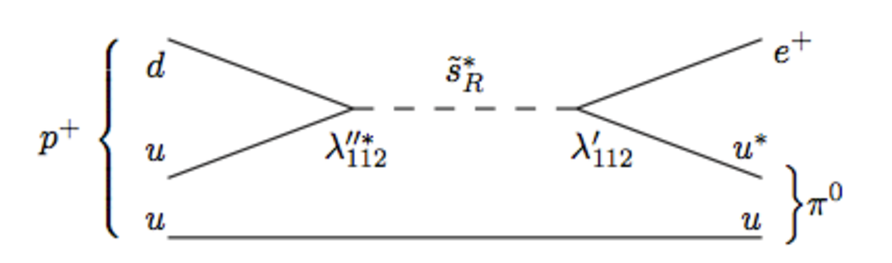
\includegraphics[scale=0.6]{figures/proton_decay.pdf}
%\caption{The Feynman diagram of proton decay. Figure adapted from \cite{Martin}.}
%\label{fig: proton decay}
%\end{center}
%\end{figure}



\section{$R$-parity}
%\subsection{$R$-parity}
%In constructing supersymmetric models, it is necessary to forbid terms in (\ref{eq: superpotential violate L}) and (\ref{eq: superpotential violate B}).
Since the superpotentials $W_{\Delta L = 1}$ and $W_{\Delta B = 1}$ are not allowed in constructing SUSY models, we introduce a new symmetry called $R$-parity which has the effect to eliminate the $B$ and $L$ violating terms while allowing all the interactions of the MSSM.
The $R$-party is defined as
\begin{equation}
R \equiv (-1)^{3(B - L) + 2s}
\end{equation}
where $s$ is the spin of the particle. All of the SM particles and the Higgs bosons have even $R$-parity ($R = +1$), while all of the sparticles have odd $R$-parity ($R = -1$).
%If the $R$-parity is conserved, there is no mixing between the sparticles and the SM particles.
If the $R$-parity is conserved, SUSY predicts that sparticles are produced in pairs in collider experiments.


\section{The lightest supersymmetric particle}
%\subsection{The lightest supersymmetric particle}
The lightest sparticle in the MSSM is called lightest supersymmetric particle (LSP), which has $R = -1$ and is absolutely stable.
Usually, LSP is electrically neutral; it doesn't join strong and electromagnetic interactions so it can be the candidate for dark matter.
Since LSP is the lightest sparticle, all other sparticles decay into a state that contains at least one LSP \footnote{Or an odd number of LSPs.} and any number of SM particles.
In collider experiments, a LSP event will look like a neutrino, which cannot be detected, and carry away some energy and momentum.
If the mass of the LSP is $m_{\widetilde{\chi}^{0}_{1}}$, the missing energy for each SUSY event will be at least $2 m_{\widetilde{\chi}^{0}_{1}}$. %because the MSSM predicts sparticles are produced in pair.













%%%%%
%%%%%
%%%%%
\chapter{Conclusion}
%\section{Conclusion}
%Maxwell combined the electricity and magnetism into electromagnetism; Salam, Glashow, and Weinberg unified electromagnetism with the weak force.
Although the SM describes the world successfully, it still cannot answer some fundamental questions such as why the coupling constants do not converge at high energy.
However, if the SM incorporates SUSY, the coupling constants do converge.
The supersymmetric version of the SM requires that every SM particle has a superpartner with a different spin.
A SM particle and its superpartner can be expressed in a supermultiplet.
Every supermultiplet contains bosons and fermions with an equal number of degrees of freedom.
There are two kinds of supermultiplets, a chiral and a vector supermultiplet.
The chiral supermultiplets can describe spin 0 and spin 1/2 particles and the vector supermultiplet can express gauge bosons and gaugions.
In the superspace, the supermultiplets are represented by superfields.
For a general superfield $S(x, \theta, \overline{\theta})$, the SUSY transformation is $(i \epsilon Q + i \overline{\epsilon} \overline{Q}) S(x, \theta, \overline{\theta})$ where $\epsilon$ is an anticommuting parameter and $Q$ is the generator of SUSY transformation.
If nature is exactly supersymmetric then the SM particles and its superpartners have the same mass.
Because we didn't find any sparticles, then SUSY must be broken spontaneously.

%Physicists are trying to construct a theory called Grand Unification Theory (GUT) which is the unification of the strong and electroweak interaction.
%The ultimate goal of physicists is to find a so-called ``theory of everything'' (ToE) which unifies the four fundamental forces in the world -- strong, electromagnetic, weak, and gravitational force.
%String theory (or Super-string theory) may turn out to be a candidate for ToE.
%SUSY plays an important role in the framework of string theory.

%There are many searches for SUSY signals, although it has not yet been found.
%If the superpartners of SM particles do exist, they may be found in the LHC when it operates at its design energy.
%We also expect that the international linear collider (ILC) and very large hadron collider (VLHC) can provide a good environment to search for SUSY signals in the long-term future. 











%%%%%
%%%%%
%%%%%

\appendix

\chapter{Superalgebra}
%\section{Superalgebra}
Since supersymmetric theory is based on superalgebra which is an extension of space-time Poincar\'{e} algebra, we first review some basic concepts of the Lorentz group, Poincar\'{e} group and spinor notation.
%We also describe the other ideas which are frequently used in the calculation of superalgebra.
At the end, we will present representations of the superalgebra, called supermultiplets.%, both massive and massless. 



\section{Lorentz group}
%\subsection{Lorentz group}
Since the Lorentz transformation combines rotations and boost, the infinitesimal Lorentz transformation matrix $U(\vec{\theta}, \vec{\phi}) $ can be written as
\begin{equation}
U(\vec{\theta}, \vec{\phi}) \simeq 1  + i \vec{\theta} \cdot \vec{J} + i \vec{\phi} \cdot \vec{K}
\end{equation}
where $\vec{\theta}$ is rotation angle, $\vec{\phi}$ is azimuth angle, and $\vec{J}$ and $\vec{K}$ are rotation and boost generators, respectively.
The generators of the Lorentz group must satisfy the commutation relations
\begin{equation}
[J_{i}, J_{j}] = i \epsilon_{ijk} J_{k}, \quad
 [K_{i}, K_{j}] = -i \epsilon_{ijk} J_{k}, \quad 
 [J_{i}, K_{j}] = i \epsilon_{ijk} K_{k}
\end{equation}
where $i, j, k = 1, 2, 3$.
It is very convenient to redefine the generators as
\begin{equation}
J^{\pm}_{i} = \frac{1}{2} (J_{i} \pm i K_{i})
\end{equation}
and the commutation relations become
\begin{equation}
[J^{+}_{i}, J^{+}_{j}] = i \epsilon_{ijk} J^{+}_{k}, \quad 
[J^{-}_{i}, J^{-}_{j}] = i \epsilon_{ijk} J^{-}_{k}, \quad 
[J^{+}_{i}, J^{-}_{j}] = 0
\end{equation}
which tell us the Lorentz group can be decomposed into the product of two independent $SU(2)$ groups.



\section{Poincar\'{e} group}
%\subsection{Poincar\'{e} group}
We need the unitary representations of a symmetry group which can preserve the translation probabilities between two eigenstates as measured in different reference frames.
The irreducible representations of the Lorentz group is not unitary, the underlying symmetry group for particle physics is the Poincar\'{e} group.
The Poincar\'{e} group is a product of the Lorentz group and the group of translations in space-time.
We usually use the energy-momentum operator $P_{\mu}$ to denote the generators of the translation groups.
If we define an antisymmetric second rank tensor generator $M_{\mu\nu}$ where the six components are the six Lorentz group generators, with $M_{ij} = \epsilon_{ijk} J_{k}$ and $M_{0i} = - M_{i0} = -K_{i}$.
Then the commutation relations of the Poincar\'{e} group are
\begin{align}
[P_{\mu}, P_{\nu}] &= 0 ,\\
[M_{\mu \nu}, P_{\lambda}] &= i (g_{\nu \lambda} P_{\mu} - g_{\mu \lambda} P_{\nu}) ,\\
[M_{\mu \nu}, M_{\rho \sigma}] &= -i (g_{\mu \rho} M_{\nu \sigma} - g_{\mu \sigma} M_{\nu \rho} - g_{\nu \rho} M_{\mu \sigma} + g_{\nu \sigma} M_{\mu \rho}) .
\end{align}
where the metric is 
%\begin{equation}
%g_{\mu \nu} = \mathrm{diag}(+1, -1, -1, -1). \notag
%\end{equation}
\[ g_{\mu \nu} =
\left(
\begin{array}{cccc}
1 & 0 & 0 & 0\\
0 & -1 & 0 & 0\\
0 & 0 & -1 & 0\\
0 & 0 & 0 & -1   
\end{array}
\right)
\]



\section{Spinors: Dirac, Magorana and Weyl fermion fields}
%\subsection{Spinors: Dirac, Magorana and Weyl fermion fields}
The general state of a spin-1/2 particle can be expressed as a two-component column matrix, called a \textbf{spinor}:
\begin{equation}
\chi = c_{+} \chi_{+} + c_{-} \chi_{-} = \left(\begin{array}{c}c_{+} \\c_{-}\end{array}\right)
\end{equation}
where $c_{+}$ and $c_{-}$ are coefficients and 
\begin{equation}
\chi_{+} = \left(\begin{array}{c}1 \\0\end{array}\right), \quad 
\chi_{-} = \left(\begin{array}{c}0 \\1\end{array}\right)
\end{equation}
representing spin up and spin down, respectively.

A \textbf{bi-spinor} is an object that consists of two spinors which belong to two different SU(2) groups.
If a four-component field $\psi_{D}$ is a solution of the Dirac equation $(i \gamma^{\mu} \partial_{\mu} - m) \psi  = 0$, we call $\psi_{D}$ a \textbf{Dirac spinor}. %which transforms under boosts and rotations according to:
%\begin{equation}
%S^{0i} = \frac{i}{4} [\gamma^{0}, \gamma^{i}] , \quad 
%S^{ij} = \frac{i}{4} [\gamma^{i}, \gamma^{j}] \equiv \frac{1}{2} \epsilon^{ijk} \Sigma^{k} .
%\end{equation}
Instead of using a four-component column matrix, we can express $\psi_{D}$ in terms of bi-spinors:
\begin{equation}
\psi_{D} = \left(\begin{array}{c} \psi_{1} \\ \psi_{2} \\ \psi_{3} \\ \psi_{4} \end{array}\right) = \left(\begin{array}{c} \psi_{L} \\ \psi_{R} \end{array}\right)
\end{equation}
where
\begin{equation}
\psi_{L} = \left(\begin{array}{c} \psi_{1} \\ \psi_{2} \end{array}\right), \quad 
\psi_{R} = \left(\begin{array}{c} \psi_{3} \\ \psi_{4} \end{array}\right)
\end{equation}
are the left-handed and right-handed \textbf{Weyl spinors}.
They transform under infinitesimal rotations $\vec{\theta}$ and boots $\vec{\beta}$ as
\begin{eqnarray}
\psi_{L} \to \psi_{L}' = (1 - i \vec{\theta} \cdot \frac{\vec{\sigma}}{2} - \vec{\beta} \cdot \frac{\vec{\sigma}}{2}) \psi_{L} ;\\
\psi_{R} \to \psi_{R}' = (1 - i \vec{\theta} \cdot \frac{\vec{\sigma}}{2} + \vec{\beta} \cdot \frac{\vec{\sigma}}{2}) \psi_{R} .
\end{eqnarray}
It is very convenient to choose the Weyl representation such that Weyl fermion fields (i.e. Weyl spinors) can be seen as the building blocks for any fermion filed.

Majorana found that if we choose all non-zero elements in all $\gamma$ matrices as purely imaginary, we can obtain a real solution $\widetilde{\psi}_{M}$ of the Dirac equation \cite{majorana}.
A Majorana fermion field is defined through the Majorana condition
\begin{equation}
\widetilde{\psi}_{M} = \widetilde{\psi}^{*}_{M} .
\end{equation}
in the Majorana representation.\footnote{We use tilde notation on the top to represent Majorana states.}
We can use similarity transformation to rewrite the Majorana condition in a general representation as
\begin{equation}
%\psi = \gamma_{0} C \psi^{*}
\psi = C \overline{\psi}^{T}
\end{equation}
which is saying a Majorana spinor is its own charge conjugate \footnote{The charge conjugation, C, converts each particle into its antiparticle: $C| \psi \rangle = | \overline{\psi} \rangle$. For $C$ can be applied to a neutral particle, and it changes the sign of all the internal quantum numbers -- charge, baryon number, lepton number, strangeness, charm, beauty, truth -- while leaving mass, energy, momentum and spin unchanged}.
We can express a Majorana fermion field in terms of left-handed and right-handed Weyl spinors
\begin{equation}
\psi_{M} = \left( \begin{array}{c} \xi_{\alpha}\\ \overline{\xi}^{\dot{\alpha}} \end{array} \right) = \left( \begin{array}{c} \xi_{\alpha}\\0\end{array} \right) + \left( \begin{array}{c}0\\ \overline{\xi}^{\dot{\alpha}} \end{array} \right) = \psi_{W, L} + \psi_{W, R}
\end{equation}
%where the right-handed Weyl spinor $\xi_{\alpha}$ is the Lorentz-covariant conjugate of the left-handed Weyl spinor.
where the right-handed Weyl spinor $\overline{\xi}^{\dot{\alpha}}$ is the Hermitian conjugate of the left-handed Weyl spinor $\xi_{\alpha}$. \footnote{The two distinct types of spinor indices $\alpha = 1, 2$ and $\dot{\alpha} = 1, 2$.}

Because the spinors anti-commute, we can derive the following identities for two spinors $\psi$ and $\chi$:
\begin{align}
& \psi \chi = \chi \psi, \quad 
\overline{\psi} \overline{\chi} = \overline{\chi} \overline{\psi}, \quad 
(\psi \chi)^{\dagger} = \overline{\psi} \overline{\chi} \notag \\
& \chi \sigma^{\mu} \overline{\psi} = - \overline{\psi} \overline{\sigma}^{\mu} \chi, \quad 
(\chi \sigma^{\mu} \overline{\psi})^{\dagger} = \psi \sigma^{\mu} \overline{\chi} \notag \\
& \chi \sigma^{\mu} \overline{\sigma}^{\nu} \psi = \psi \sigma^{\nu} \overline{\sigma}^{\mu} \chi, \quad 
(\chi \sigma^{\mu} \overline{\sigma}^{\nu} \psi)^{\dagger} = \overline{\psi} \overline{\sigma}^{\nu} \sigma^{\mu} \overline{\chi}
\end{align}



\section{Helicity and chirality}
%\subsection{Helicity and chirality}
Both helicity and chirality mean ``handedness". %but they are slightly different.
Helicity is the projection of angular momentum $\vec{J}$ onto the direction of momentum $\hat{p}$.
Since the orbital angular momentum $\vec{L}$ is perpendicular to the direction of momentum, it therefore does not contribute to helicity.
\begin{equation}
h = \vec{J} \cdot \hat{p} = (\vec{L} + \vec{S}) \cdot \hat{p} = \vec{S} \cdot \hat{p}, \quad 
\hat{p} = \frac{\vec{p}}{|\vec{p}|}
\end{equation}
It can be easily seen that the eigenvalues of $h$ are $\pm 1$.
An eigenstate with eigenvalue $-1$ is called ``left-handed" and an eigenstate with eigenvalue $+1$ is called ``right-handed" as shown in figure \ref{fig: helicity}.
\begin{figure}
\centering
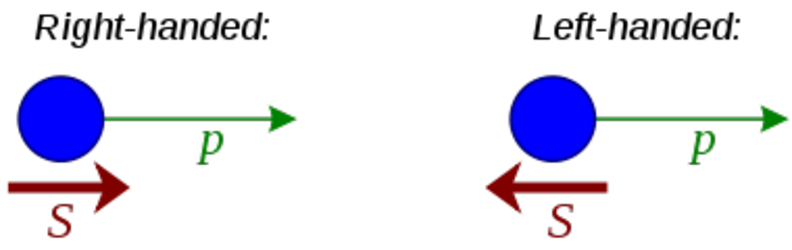
\includegraphics[scale=0.8]{figures/380px-Right_left_helicity.pdf}
%This figure is from http://commons.wikimedia.org/wiki/File:Right_left_helicity.svg
\caption{Helicity. On the left hand side, spin and momentum are parallel (helicity $+1$); on the right hand side they are antiparallel (helicity $-1$) \cite{helicity}.} %Figure adapted from \url{http://commons.wikimedia.org/wiki/File:Right\_left\_helicity.svg}.}
\label{fig: helicity}
\end{figure}
Although helicity is invariant under rotations, it is not invariant under boosts.
The only exception is when particles are massless, the helicity is Lorentz invariant because massless particles would move at the speed of light.

The chirality is related to the matrix $\gamma_{5}$ which is defined as
\begin{equation}
\gamma_{5} = \gamma^{5} \equiv i \gamma^{0} \gamma^{1} \gamma^{2} \gamma^{3}
\end{equation}
and has the following properties
\begin{equation}
\{ \gamma_{5}, \gamma_{\mu} \} = 0, \quad 
\gamma_{5}^{\dagger} = \gamma_{5}, \quad 
(\gamma_{5})^{2} = 1
\end{equation}
where the $\gamma$ matrices are defined in \cite{peskin_qft.}
The chirality operators are defined as
\begin{equation}
P_{L} = \frac{1 - \gamma_{5}}{2}, \quad 
P_{R} = \frac{1 + \gamma_{5}}{2}
\end{equation}
A particle bi-spinor $\psi$ consists of left-chiral and right-chiral parts,
\begin{equation}
\psi = \psi_{L} + \psi_{R}
\end{equation}
where
\begin{equation}
\psi_{L} = P_{L} \psi, \quad 
\psi_{R} = P_{R} \psi
\end{equation}
It is easy to show that $P_{L} \psi_{R} = 0$ and $P_{R} \psi_{L} = 0$.
The chirality of the field has the property that a left-chiral solution of the Dirac equation remains left-chiral under Lorentz transformations and likewise for a right-chiral field.
Since $\gamma_{5}$ anticommutes with all the other $\gamma$ matrices, the chirality is not conserved because of the mass term in the Dirac Hamiltonian $H = \gamma^{0} (\gamma^{i} p_{i} + m)$.
If we are considering massless particles, the difference between helicity and chirality disappears  \cite{arXiv:1006.1718v2}.
%The relation between helicity and chirality for massless particles can be found in Ref. \cite{arXiv:1006.1718v2}.



\section{Grassmann numbers}
%\subsection{Grassmann numbers}
The Grassmann numbers are anticommuting objects
\begin{equation}
\{\theta_{\alpha}, \theta_{\beta}\} = \{\overline{\theta}_{\dot{\alpha}}, \overline{\theta}_{\dot{\beta}}\} = \{\theta_{\alpha}, \overline{\theta}_{\dot{\beta}}\} = 0
\end{equation}
where $\alpha, \beta, \dot{\alpha}$, and $\dot{\beta} = 1, 2$ \footnote{$\overline{\theta}_{\dot{\alpha}}$ = $\theta_{\alpha}^{\dagger}$ }
%\footnote{The $\theta_{\alpha}$ and $\overline{\theta}_{\dot{\alpha}}$ are two distinct constant spinors. They are not the complex conjugate.}.
We can easily prove the following identities:
\begin{align}
&\theta_{\alpha} \theta_{\beta} = \frac{1}{2} \epsilon_{\alpha \beta} \theta \theta, \quad 
\overline{\theta}_{\dot{\alpha}} \overline{\theta}_{\dot{\beta}} = -\frac{1}{2} \epsilon_{\dot{\alpha} \dot{\beta}} \overline{\theta} \overline{\theta}, \quad 
\theta_{\alpha} \overline{\theta}_{\dot{\beta}} = \frac{1}{2} \sigma^{\mu}_{\alpha \dot{\beta}} (\overline{\theta} \overline{\sigma}_{\mu} \theta) \notag \\
& (\theta \psi)(\theta \chi) = - \frac{1}{2}\theta \theta \psi \chi, \quad 
(\overline{\theta} \overline{\psi})(\overline{\theta} \overline{\chi}) = - \frac{1}{2} \overline{\theta} \overline{\theta} \overline{\psi} \overline{\chi}, \quad 
(\theta \psi)(\overline{\theta} \overline{\chi}) = \frac{1}{2}(\overline{\theta} \overline{\sigma}^{\mu} \theta)(\psi \sigma_{\mu} \overline{\chi}) \notag \\
& (\theta \sigma^{\mu} \overline{\theta})(\theta \sigma^{\nu} \overline{\theta}) = \frac{1}{2} \theta \theta \overline{\theta} \overline{\theta} g^{\mu \nu} .
\end{align}
Derivatives with respect to the Grassmann numbers are defined by
\begin{equation}
\frac{\partial}{\partial \theta^{\alpha}}(\theta^{\beta}) = \delta^{\beta}_{\alpha}, \quad
\frac{\partial}{\partial \overline{\theta}_{\dot{\alpha}}}(\overline{\theta}_{\dot{\beta}}) = \delta^{\dot{\alpha}}_{\dot{\beta}}, \quad 
\frac{\partial}{\partial \theta^{\alpha}}(\overline{\theta}_{\dot{\beta}}) = 0, \quad 
\frac{\partial}{\partial \overline{\theta}_{\dot{\alpha}}}(\theta^{\beta}) = 0
\end{equation}
and the integrations are defined as
\begin{equation}
\int d\theta_{\alpha} = 0, \quad 
\int d\theta_{\alpha} \ \theta_{\alpha}  = 1 .
\end{equation}
If we have a general function $f$ which is linear in $\theta_{\alpha}$:
\begin{equation}
f(\theta_{\alpha}) = f_{0} + \theta_{\alpha} f_{1} ,
\end{equation}
where $f_{0}$ and $f_{1}$ can be functions of other commuting or anticommuting variables but not functions of $\theta_{\alpha}$.
We can find differentiation and integration give the same results for Grassmann numbers
\begin{equation}
\frac{df}{d\theta_{\alpha}} = f_{1}, \quad \int d\theta_{\alpha} f(\theta_{\alpha}) = f_{1} .
\end{equation}
We also define
\begin{equation}
d^{2} \theta = \frac{1}{2} d\theta^{1} d\theta^{2}, \quad  
d^{2}\overline{\theta} = \frac{1}{2} d\overline{\theta}^{2} d\overline{\theta}^{1} = (d^{2} \theta)^{\dag}
\end{equation}
such that
\begin{equation}
\int d^{2} \theta \ \theta \theta = \int d^{2} \overline{\theta} \ \overline{\theta} \overline{\theta} = 1 .
\end{equation}



\section{Supermultiplets} \label{sec: supermultiplets}
%\subsection{Supermultiplets} \label{sec: supermultiplets}
The enlarged Poincar\'{e} group, called super-Poincar\'{e} group, has generators $Q^{I}_{\alpha}$ and its conjugate $\overline{Q}^{I}_{\dot{\alpha}}$ which obey the commutation relations
\begin{align}
& [P_{\mu}, Q^{I}_{\alpha}] = 0, \quad 
[P_{\mu}, \overline{Q}^{I}_{\dot{\alpha}}] = 0,\\
& [M_{\mu \nu}, Q^{I}_{\alpha}] = i {(\sigma_{\mu \nu})_{\alpha}}^{\beta} Q^{I}_{\beta}, \quad 
[M_{\mu \nu}, \overline{Q}^{I\dot{\alpha}}] = i {(\overline{\sigma}_{\mu \nu})^{\dot{\alpha}}}_{\dot{\beta}} \overline{Q}^{I \dot{\beta}}\\
& \{Q^{I}_{\alpha}, \overline{Q}^{J}_{\dot{\beta}}\} = 2 \sigma^{\mu}_{\alpha \dot{\beta}} P_{\mu} \delta^{IJ}\\
& \{Q^{I}_{\alpha}, Q^{J}_{\beta}\} = \epsilon_{\alpha \beta} Z^{IJ}, \quad 
\{\overline{Q}^{I}_{\dot{\alpha}}, \overline{Q}^{J}_{\dot{\beta}}\} = \epsilon_{\dot{\alpha} \dot{\beta}} (Z^{IJ})^{*}
\end{align}
where $I, J = 1, \dots, N$ and the central charge $Z^{IJ} = -Z^{JI}$ is nonvanishing only for $N > 1$ and commutes with all generators.
Although there is no upper limit on $N$ from the algebraic point of view, $N$ must be less than or equal to $8$ in order to have physical meaning.
We only discuss the simplest case $N = 1$. %and do not talk about the extended SUSY ($N > 1$) case.

From the commutation relations listed above, it is easy to show that $[J_{3}, Q^{I}_{1}] = \frac{1}{2} Q^{I}_{1}$ and $[J_{3}, Q^{I}_{2}] = - \frac{1}{2} Q^{I}_{2}$.
Similarly, $[J_{3}, (Q^{I}_{1})^{\dag}] = -\frac{1}{2} (Q^{I}_{1})^{\dag}$ and $[J_{3}, (Q^{I}_{2})^{\dag}] = \frac{1}{2} (Q^{I}_{2})^{\dag}$.
Hence we can conclude that $Q^{I}_{1}$ and $(Q^{I}_{2})^{\dag}$ raise the z-component of the spin (helicity) by $\frac{1}{2}$ and $Q^{I}_{2}$ and $(Q^{I}_{1})^{\dag}$ lower it by $\frac{1}{2}$.

The single particle states of a SUSY theory correspond to irreducible representations of super-Poincar\'{e} algebra, called supermultiplets.
Every supermultiplet contains both bosons and fermions with an equal number of degrees of freedom; and all particles belonging to the same supermultiplet have the same mass because $P^{2}$ commutes with all generators of the SUSY algebra.
If we consider a massless supermultiplet in unextended SUSY ($N = 1$), than there are three kinds of multiplets:
$(0, \frac{1}{2}) \otimes (-\frac{1}{2}, 0)$, the chiral multiplet, which contains a complex scalar and a Weyl fermion;
$(\frac{1}{2}, 1) \otimes (-1, -\frac{1}{2})$, the vector multiplet, which contains a gauge boson and a Weyl fermion;
$(\frac{3}{2}, 2) \otimes (-2, -\frac{3}{2})$, the graviton multiplet, which contains a graviton and a gravitino.

For a massive case, there are 4 states, labeled by their helicities (or rather the $z$ component of the angular momentum): $(-\frac{1}{2}, 0, 0, \frac{1}{2})$ and the same for its CPT conjugate $(-\frac{1}{2}, 0, 0, \frac{1}{2})$, and $(-1, -\frac{1}{2}, -\frac{1}{2}, 0)$ and its CPT conjugate $(1, \frac{1}{2}, \frac{1}{2}, 0)$.
The detailed discussions about massless and massive supermultiplets can be found in many references such as \cite{Bilal} and \cite{larsenf}.





%%%%%
%%%%%
%%%%%
\chapter{Supersymmetric gauge theories}
%\section{Supersymmetric gauge theories}

Since all the known interactions are gauge interactions, we have to extend gauge interactions to their supersymmetric version.
This can be divided into two cases, one for Abelian and one for non-Abelian.



\section{Lagrangians for gauge superfields}
%\subsection{Lagrangians for gauge superfields}
A vector superfield V which is used to describe the gauge bosons contains a massless gauge boson field $A^{a}_{\mu}$ \footnote{The field $A^{\mu}$ is defined as $(V, \vec{A})$ which is the conventions in electrodynamics.} and a gaugino field $\lambda^{a}$.
Under the gauge transformation, they transform as
\begin{align}
& A^{a}_{\mu} \to A^{a}_{\mu} + \partial_{\mu} \Lambda^{a} + g f^{abc} A^{b}_{\mu} \Lambda^{c} ,\\
& \lambda^{a} \to \lambda^{a} + g f^{abc} \lambda^{b} \Lambda^{c}
\end{align}
where $\Lambda^{a}$ is an infinitesimal gauge transformation parameter, $g$ is the gauge coupling constant, and $f^{abc}$ is the antisymmetric structure constant of the gauge group.
Because gauge transformation removes one degree of freedom from $A^{a}_{\mu}$, we have to introduce a real bosonic auxiliary field $D^{a}$.
This gauge auxiliary field has mass dimension 2 and no kinetic term, so it can be eliminated using the equation of motion.
The Lagrangian density of a gauge superfield is
\begin{equation} \label{eq: L_gauge}
\mathcal{L}_{\mathrm{gauge}} = - \frac{1}{4} F^{a}_{\mu \nu} F^{\mu \nu a} + i \lambda^{\dag a} \overline{\sigma}^{\mu} \nabla_{\mu} \lambda^{a} + \frac{1}{2} D^{a} D^{a} ,
\end{equation}
where the gauge field strength $F^{a}_{\mu \nu}$ is defined as
\begin{equation} \label{eq: gauge field strength}
F^{a}_{\mu \nu} = \partial_{\mu} A^{a}_{\nu} - \partial_{\nu} A^{a}_{\mu} + g f^{abc} A^{b}_{\mu} A^{c}_{\nu}
\end{equation}
and
\begin{equation}
\nabla_{\mu} \lambda^{a} = \partial_{\mu} \lambda^{a} + g f^{abc} A^{b}_{\mu} \lambda^{c}
\end{equation}
is the covariant derivative of the gaugino field.
If we apply SUSY transformation to the fields $A^{a}_{\mu}$, $\lambda^{a}$, and $D^{a}$, we can find the $\mathcal{L}_{\mathrm{gauge}}$ is supersymmetric.



\section{Supersymmetric gauge interactions}
%\subsection{Supersymmetric gauge interactions}
When gauge interactions are involved, we have to promote the ordinary derivative to a gauge-covariant derivative
\begin{equation}
\partial_{\mu} \psi_{i} \to \nabla_{\mu} \psi_{i} = \partial_{\mu} \psi_{i} - i g_{a} A^{a}_{\mu} T^{aj}_{i} \psi_{j}
\end{equation}
where $g_{a}$ is the gauge coupling, $T^{a}$ is the generator matrix, and $A^{a}_{\mu}$ is the vector field.
And the SUSY transformations are modified to
\begin{align} \label{eq: total Lagrangian}
\delta \phi_{i} &= \epsilon \psi_{i}\\
\delta (\psi_{i})_{\alpha} &= - i (\sigma^{\mu} \epsilon^{\dag})_{\alpha} \nabla_{\mu} \phi_{i} + \epsilon_{\alpha} F_{i}\\
\delta F_{i} &= -i \epsilon^{\dag} \overline{\sigma}^{\mu} \nabla_{\mu} \psi_{i} + \sqrt{2} g (T^{a} \phi)_{i} \epsilon^{\dag} \lambda^{\dag a}
\end{align}
With the help of the extra term $\sqrt{2} g (T^{a} \phi)_{i} \epsilon^{\dag} \lambda^{\dag a}$ in $\delta F_{i}$, the total Lagrangian density
\begin{align} \label{eq: Lagrangian for gauge theory}
\mathcal{L} &= \nabla^{\mu} \phi^{*i} \nabla_{\mu} \phi_{i} + i \psi^{\dag i} \overline{\sigma}^{\mu} \nabla_{\mu} \psi_{i} -\frac{1}{2} \Big( W^{ij} \psi_{i} \psi_{j} + W^{*}_{ij} \psi^{\dag i} \psi^{\dag j} \Big) - W^{i} W^{*}_{i} \notag \\
& -\frac{1}{4} F^{a}_{\mu \nu} F^{\mu \nu a} + i \lambda^{\dag a} \overline{\sigma}^{\mu} \nabla_{\mu} \lambda^{a} + \frac{1}{2} D^{a} D^{a} \notag \\
& -\sqrt{2} g (\phi^{*} T^{a} \psi) \lambda^{a} - \sqrt{2} g \lambda^{\dag a} (\psi^{\dag} T^{a} \phi) + g(\phi^{*} T^{a} \phi) D^{a}
\end{align}
is invariant under the SUSY transformations.
From this Lagrangian, we can combine the $D^{a} D^{a} / 2$ term with $g (\phi^{*} T^{a} \phi) D^{a}$ to find the equations of motion for the auxiliary field $D^{a}$
\begin{equation} \label{eq: E.O.M of D field}
D^{a} = - g (\phi^{*} T^{a} \phi) .
\end{equation}
Replacing the auxiliary field in (\ref{eq: total Lagrangian}) using (\ref{eq: E.O.M of D field}), we can find that the scalar potential is
\begin{equation} \label{eq: scalar potential}
V(\phi, \phi^{*}) = F^{*i} F_{i} + \frac{1}{2} \sum_{a} D^{a} D_{a} = W^{i} W^{*}_{i} + \frac{1}{2} \sum_{a} g^{2}_{a} (\phi^{*} T^{a} \phi)^{2} .
\end{equation}
Since $V(\phi, \phi^{*})$ is a sum of square terms and it is non-negative.



\section{Superspace Lagrangians for Abelian and non-Abelian gauge theory}
%\subsection{Superspace Lagrangians for Abelian and non-Abelian gauge theory}
Although we have obtained the Lagrangian for Abelian gauge theory in (\ref{eq: Lagrangian for gauge theory}), there is another way to compute the Lagrangians using the gauge-invariant Abelian field strength superfields which is defined as
\begin{equation}
W_{\alpha} = -\frac{1}{4} \overline{D} \overline{D} D_{\alpha} V, \quad
\overline{W}_{\dot{\alpha}} = -\frac{1}{4} D D \overline{D}_{\dot{\alpha}}
\end{equation}
with mass dimension $3/2$.
Since $D^{3} = \overline{D}^{3} = 0$, from (\ref{eq: definition of chiral superfield}) and (\ref{eq: definition of antichiral superfield}) we know $W_{\alpha}$ is chiral and $\overline{W}_{\dot{\alpha}}$ is antichiral.
Because $W_{\alpha}$ is gauge invariant, the easiest way to derive the general expression is using the Wess-Zumino gauge.
After converting the vector superfields V in (\ref{eq: WZ gauge vector superfield}) to $(y^{\mu}, \theta_{\alpha}, \overline{\theta}_{\dot{\alpha}})$ coordinate, we get
\begin{equation}
V (y, \theta, \overline{\theta}) |_{\mathrm{WZ}} = \theta \sigma^{\mu} \overline{\theta} A_{\mu} (y) + i \theta \theta \overline{\theta} \overline{\lambda} (y) - i \overline{\theta} \overline{\theta} \theta \lambda (y) + \frac{1}{2} \theta \theta \overline{\theta} \overline{\theta} [ D(y) - i \partial_{\mu} A^{\mu} (y) ]
\end{equation}
and
\begin{equation} \label{eq: field strength chiral superfield in abelian gauge}
W_{\alpha} = -i \lambda_{\alpha} (y) + \theta_{\alpha} D(y) + \frac{i}{2} (\sigma^{\mu} \overline{\sigma}^{\nu} \theta)_{\alpha} F_{\mu \nu} (y) - i \theta \theta (\sigma^{\mu} \partial_{\mu} \overline{\lambda} (y))_{\alpha}
\end{equation}
where $F_{\mu \nu}$ is the field strength.
Since $W_{\alpha}$ is a chiral superfield, we can calculate the SUSY invariant Lagrangian
\begin{equation}
\mathcal{L} = \int d^{2} \theta \ \frac{1}{4} [W^{\alpha} W_{\alpha}] + c.c = \frac{1}{2} D^{2} + i \overline{\lambda} \overline{\sigma}^{\mu} \partial_{\mu} \lambda - \frac{1}{4} F^{\mu \nu} F_{\mu \nu}
\end{equation}
and agree with (\ref{eq: L_gauge}).

For a non-Abelian gauge group, the vector superfields transform as
\begin{align}
e^{V} &\to e^{i \Lambda^{\dag}} e^{V} e^{-i \Lambda}\\
e^{-V} & \to e^{i \Lambda} e^{-V} e^{-i \Lambda^{\dag}}
\end{align}
and the field strength chiral superfield becomes
\begin{equation}
W_{\alpha} = -\frac{1}{4} \overline{D} \overline{D} (e^{-V} D_{\alpha} e^{V})
\end{equation}
and it transforms under supergauge transformations as
\begin{equation}
W_{\alpha} \to e^{i \Lambda} W_{\alpha} e^{-i \Lambda}.
\end{equation}
After applying Wess-Zumino gauge, the component expansion of $W_{\alpha}$ is
\begin{equation}
W_{\alpha} = -i \lambda_{\alpha} (y) + \theta_{\alpha} D(y) + \frac{i}{2} (\sigma^{\mu} \overline{\sigma}^{\nu} \theta)_{\alpha} F_{\mu \nu} (y) - i \theta \theta (\sigma^{\mu} \nabla_{\mu} \overline{\lambda} (y))_{\alpha}
\end{equation}
which is the same as (\ref{eq: field strength chiral superfield in abelian gauge}) except the ordinary derivatives of the field turn into gauge corivant derivatives and the gauge field strength $F_{\mu \nu}$ is defined in (\ref{eq: gauge field strength}).
If we introduce complex coupling constant
\begin{equation}
\tau = \frac{\Theta}{2 \pi} + \frac{4 \pi i}{g^{2}}
\end{equation}
where $g$ is the gauge coupling constant and $\Theta$ is $\Theta$-angle.
Then the general Lagrangian for supersymmetric gauge theory is
\begin{align}
\mathcal{L} &= \frac{1}{32 \pi} \Im (\tau \int d^{2} \theta \ \mathrm{Tr} W^{\alpha} W_{\alpha}) \notag\\
&= \mathrm{Tr} \big( -\frac{1}{4} F_{\mu \nu} F^{\mu \nu} -i \lambda \sigma^{\mu} D_{\mu} \overline{\lambda} + \frac{1}{2} D^{2} \big)
+ \frac{\Theta}{32 \pi^{2}} g^{2} \ \mathrm{Tr} F_{\mu \nu} \widetilde{F}^{\mu \nu}
\end{align}
where $\widetilde{F}^{\mu \nu}$ is the dual field strength
\begin{equation}
\widetilde{F}^{\mu \nu} = \frac{1}{2} \epsilon^{\mu \nu \rho \sigma} F_{\rho \sigma} .
\end{equation}






%%%%%
%%%%%
%%%%%
\chapter{The search for supersymmetry}
%\section{The search for supersymmetry}
%9612229v2.pdf \cite{Dawson}
%0000388.pdf \cite{Haber and Kane}
%$0034-4885_69_11_R01$.pdf \cite{Pape and Treille}

%Although the current experimental study of SUSY is setting limits because we haven't find any SUSY signal yet, scientists hope that the evidences of SUSY signals can be found when LHC powers up to 14TeV.
The large hadron collider (LHC) is a proton-proton collider with centre of mass energy up to 14 TeV.
The LHC was built to search for Higgs bosons but it also has potential to probe new physics beyond the SM.
If the predictions of SUSY theories were correct, we might find sparticles produced by the LHC.
ATLAS and CMS experiments are two of the four important experiments at the LHC and the current SUSY status will be described for both experiment below.



\section{SUSY in ATLAS}
%\subsection{SUSY in ATLAS}
The ATLAS detector consists of inner detector, calorimeter, muon detector, and magnetic system.
The inner detector gives accurate momentum and vertex measurements, the calorimeters have excellent energy and position resolutions for charged particles, and the muon detector measures the energy of mouns. %as they pass through.
More details about the ATLAS detector can be found in Ref. \cite{atlas_detector}.
If $R$-parity is conserved, SUSY predicts that sparticles are produced in pairs in collider experiments and all heavy sparticles must decay to a state with an odd number of LSP.
The ATLAS collaboration can use the events with multiple leptons and missing transverse energy from LSP in the final state to search charginos \footnote{Chargions $\widetilde{\chi}^{\pm}_{1, 2}$ are the mass eigenstates of the charged higgsino and charged winos.}, neutralinos \footnote{Neutralinos $\widetilde{\chi}^{0}_{1,2,3,4}$ are the mass eigenstates of the neutral gauginos and neutral higgsinos.}, and sleptons in ATLAS.

Since a typical SUSY model involves many sparticles with different masses and there are different possible ways for each to decay, we have to simplify the models to study a specific decay chain with the assumed branching ratio.
We also need to understand and accurately model the SM background because the SM processes can mimic the SUSY signal.
The background can be reducible or irreducible, where the irreducible background has the same final state as signal.
The main backgrounds are $W/Z + \mathrm{jets}$, $t \overline{t}$, and di-bosons events.
Several methodologies were developed to model the possible backgrounds.
%Several methodologies, for example, matrix method and monte carlo, were developed to model the possible backgrounds.
So far, there is no evidence for SUSY has been observed with the dataset collected by ATLAS.
Figure \ref{fig: ATLAS_SUSY_Summary} shows the newest SUSY research at ATLAS.
If SUSY does exist at the TeV scale, the signals can be found when the LHC operates at higher energy.
\begin{figure}[htbp]
\begin{center}
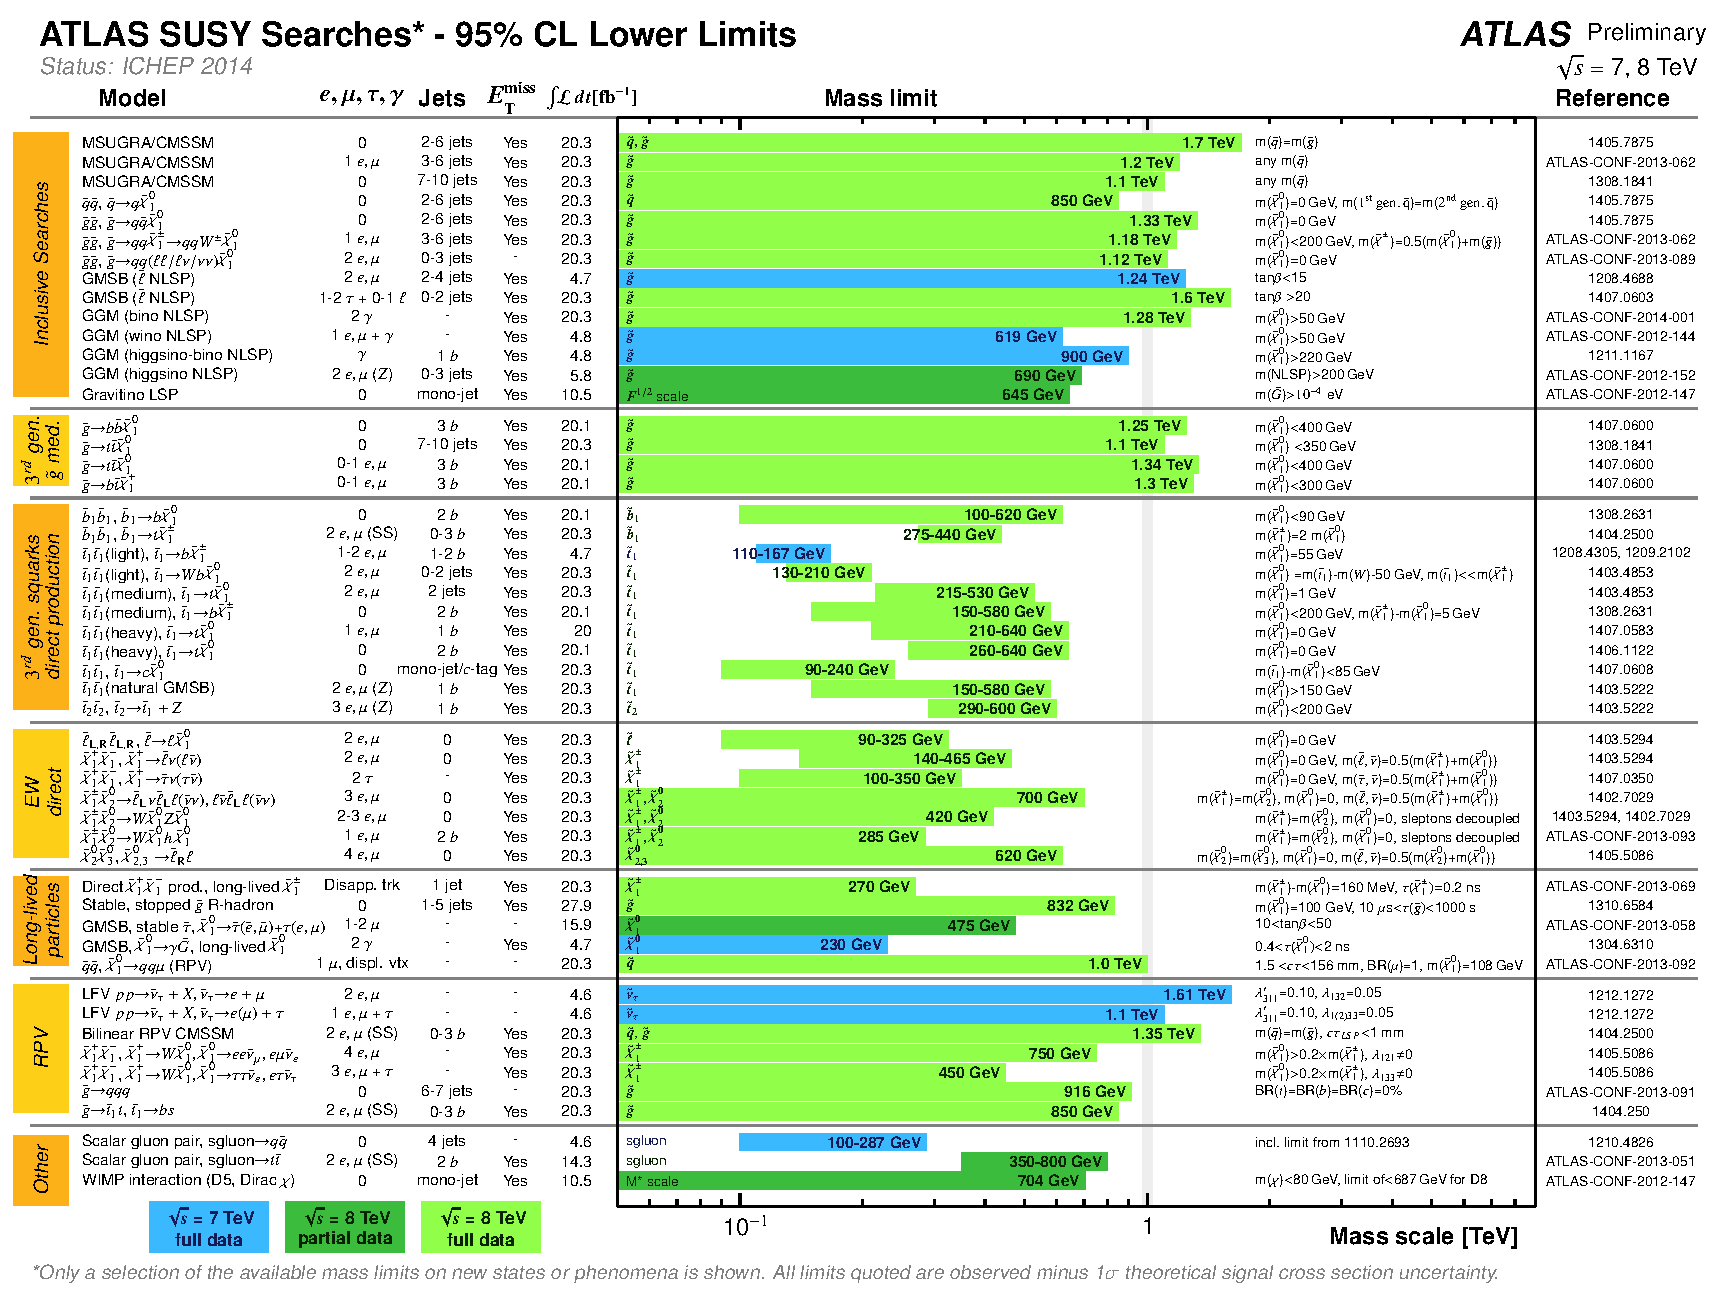
\includegraphics[scale=0.6]{figures/ATLAS_SUSY_Summary.pdf}
\caption{The mass limits of sparticles in the ATLAS SUSY searches with $95\%$ confidence level \cite{atlas_results}.} %Figure adapted from \url{https://twiki.cern.ch/twiki/bin/view/AtlasPublic/SupersymmetryPublicResults}.}
\label{fig: ATLAS_SUSY_Summary}
\end{center}
\end{figure}


\section{SUSY in CMS}
%\subsection{SUSY in CMS}
Similar to the ATLAS detector, the Compact Muon Solenoid (CMS) particle detector is a general-purpose detector at LHC.
The central feature of the CMS apparatus is a superconducting solenoid, of 6 m internal diameter, providing a magnetic field of 3.8 T.
Within the magnetic field volume are a silicon pixel and strip tracker, a crystal electromagnetic calorimeter, and a brass-scintillator hadron calorimeter.
Muons are measured in gas-ionization detectors embedded in the steel flux-return yoke located outside the solenoid.
A detailed description of the CMS detector can be found in Ref. \cite{cms_detector}.
%Like a cylindrical onion, the CMS detector consists of layers of material which can record the path, momentum, and energy of particles with accurate precision.
%The silicon tracker, superconducting solenoid magnet, crystal calorimeter, hadron calorimeter, and muon chamber.
Although the CMS experiment has similar scientific goals as the ATLAS experiment, it has different design in the detector and might use different methods to analyse the collected data.
The CMS experiment doesn't find any sparticles but it provides the limits for some possible channel as shown in figure \ref{fig: barplot_ICHEP2014}.
\begin{figure}[htbp]
\begin{center}
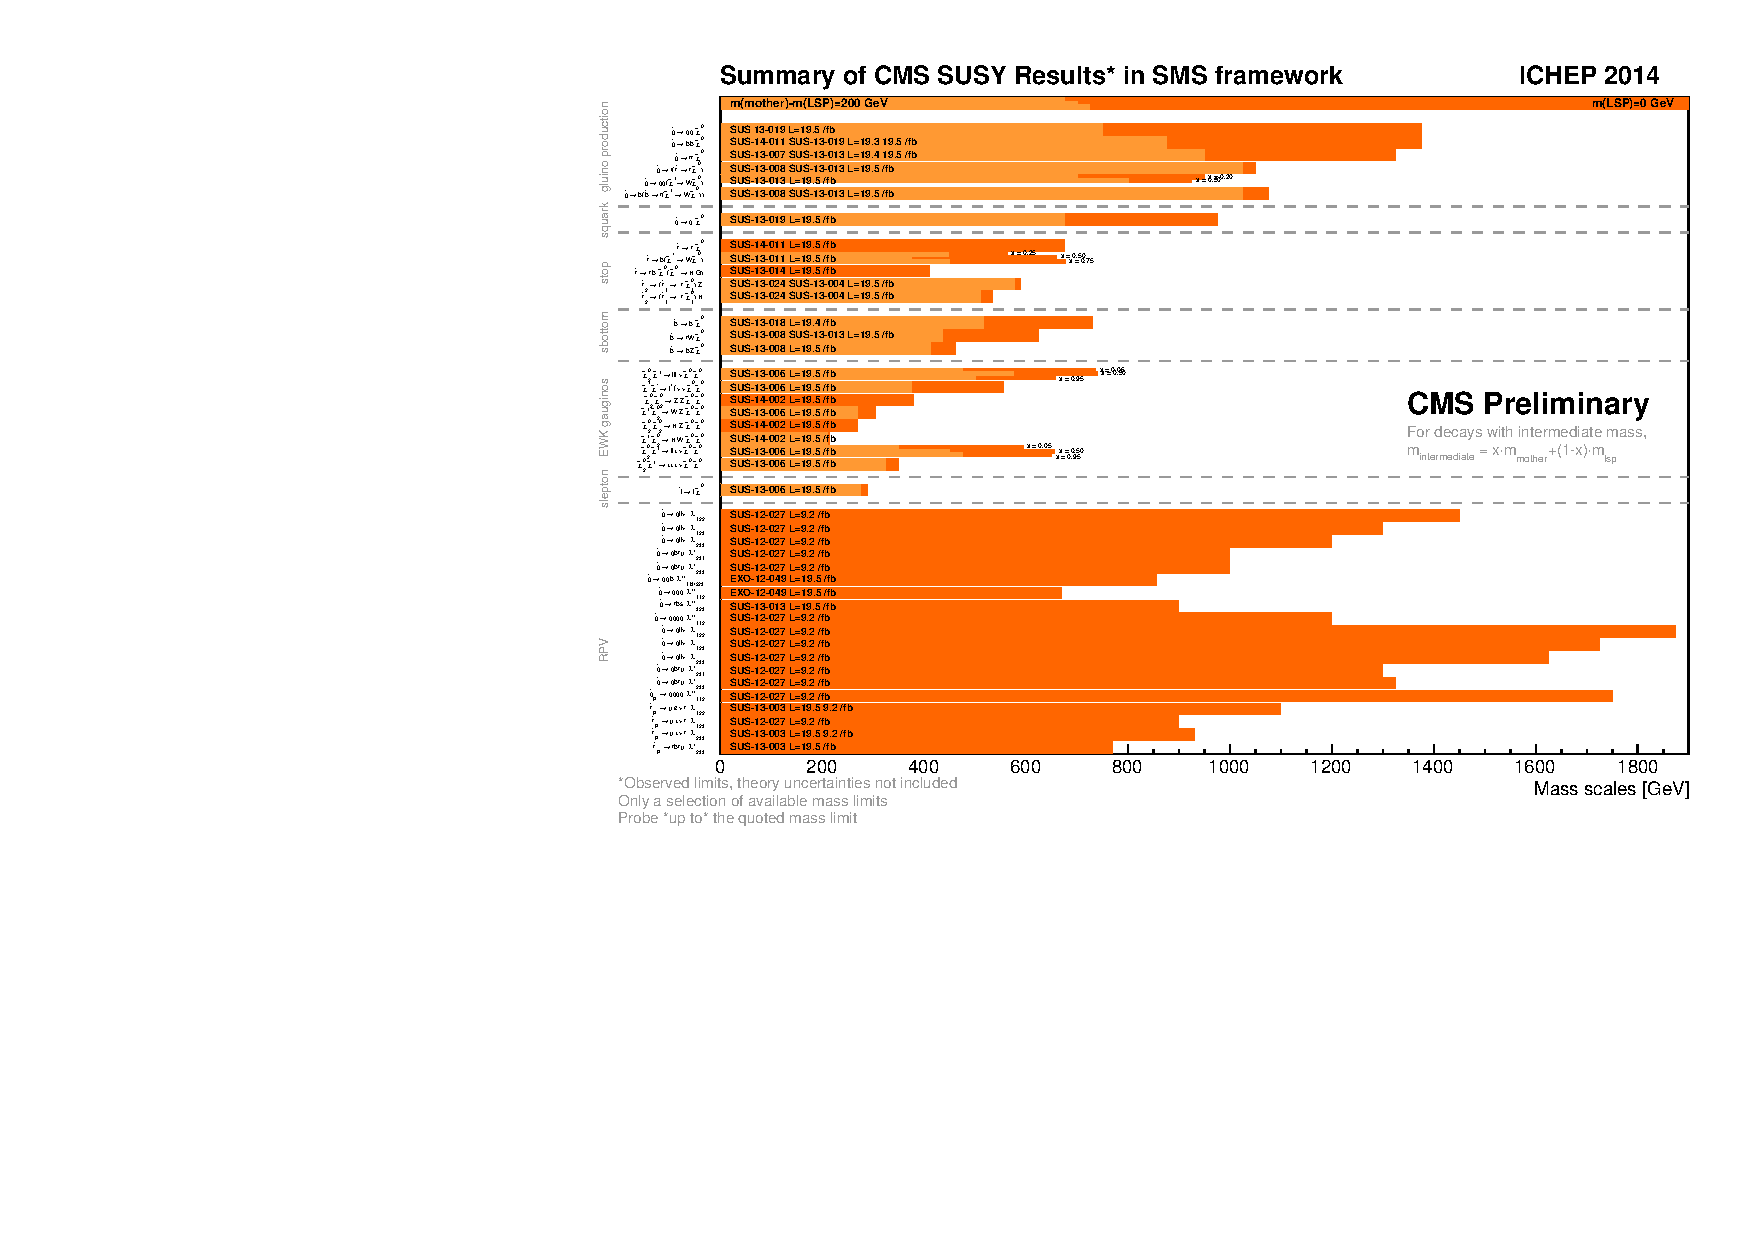
\includegraphics[scale=0.8]{figures/barplot_ICHEP2014.pdf}
\caption{The exclusion limits for the masses of the mother particles for $\mathrm{m(LSP)} = 0 \ GeV$ (dark shades) and $\mathrm{m(mother)} - \mathrm{m(LSP)} = 200 \ GeV$ (light shades), for all results \cite{cms_results}.} %Figure adapted from \url{https://twiki.cern.ch/twiki/bin/view/CMSPublic/SUSYSMSSummaryPlots8TeV}.}
\label{fig: barplot_ICHEP2014}
\end{center}
\end{figure}







% bibliography 
\bibliographystyle{unsrt}
\bibliography{specialist}



%\begin{thebibliography}{999}
%\bibitem{wess_and_zumino} Wess, J.; Zumino, B. (1974). "Supergauge transformations in four dimensions". Nuclear Physics B 70 (1): 39 $-$ 50.
%\bibitem{running_coupling_constants} \url{http://www.nobelprize.org/nobel_prizes/physics/laureates/2004/phypub4highen.jpg}
%%\bibitem{the_composition_of_the_universe} Figure adapted from http://wmap.gsfc.nasa.gov/news/
%\bibitem{majorana} E. Majorana (1937), "Theory of the symmetry of electrons and positrons", Nuovo Cim. 14 (1937): 171 $-$184.
%\bibitem{helicity} \url{http://commons.wikimedia.org/wiki/File:Right\_left\_helicity.svg}
%\bibitem{arXiv:1006.1718v2} Palash B. Pal (2010). "Dirac, Majorana and Weyl fermions". arXiv:1006.1718v2 [hep-ph] 12 Oct 2010.
%\bibitem{Bilal} Adel Bilal. "Introduction to Supersymmetry". arXiv:hep-th/0101055v1 10 Jan 2001.
%\bibitem{larsenf} \url{http://www-personal.umich.edu/~larsenf/Lecture1.pdf}
%\bibitem{Martin} Stephen Martin. "A Supersymmetry Primer". arXiv:hep-ph/9709356v6 6 Sep 2011.
%\bibitem{Pesink} Michael Peskin. "Supersymmetry in Elementary Particle Physics". arXiv:0801.1928 [hep-ph] 13 Jan 2008.
%\bibitem{Drees} Manuel Dress. "An Introduction to Supersymmetry". arXiv:hep-ph/9611409v1 25 Nov 1996.
%\bibitem{O_Raifeartaigh} L. O'Raifeartaigh. '' Nucl. Phys. B \textbf{96}, 331 (1975)
%\bibitem{atlas_detector} ATLAS Collaboration, The ATLAS Experiment at the CERN Large Hadron Collider, JINST 3 (2008) S08003 doi:10.1088/1748-0221/3/08/S08003
%%\url{https://twiki.cern.ch/twiki/pub/Atlas/AtlasTechnicalPaper/Published_version_jinst8_08_s08003.pdf}
%\bibitem{cms_detector} CMS Collaboration, The CMS experiment at the CERN LHC, JINST 3 (2008) S08004, doi:10.1088/1748-0221/3/08/S08004.
%\bibitem{atlas_results} \url{https://twiki.cern.ch/twiki/bin/view/AtlasPublic/SupersymmetryPublicResults}
%\bibitem{cms_results} \url{https://twiki.cern.ch/twiki/bin/view/CMSPublic/SUSYSMSSummaryPlots8TeV}
%\bibitem{peskin_qft} Equations (3.41) and (3.42) in ``An Introduction to Quantum Field Theory'' written by Peskin and Schroeder.
%%\bibitem{Dawson} S. Dawson. "Susy and such". arXiv:hep-ph/9612229v2 14 Jan 1997
%%\bibitem{Aitchison} Ian J. R. Aitchison. "Supersymmetry in Particle Physics An Elementary Introduction". SLAC-R-865 May 2007
%%\bibitem{Haber and Kane} Howard E. Haber; G.L. Kane. "The search for supersymmetry: probing physics beyond the standard model"
%%\bibitem{Pape and Treille} Lue Pape; Daniel Treille. "Supersymmetry facing experiment: much ado (already) about nothing (yet)". Rep. Prog. Phys. \textbf{69} (2006) 2843-3067
%%\bibitem{Jungman, Kamionkowski, Griest} Gerard Jungman, Marc Kamionkowski, Kim Griest. "Supersymmetric dark matter". Physics Reports 267 (1996) 195-373
%\end{thebibliography}



\end{document}